\documentclass[a4paper]{article}
\usepackage[T1]{fontenc}
\usepackage{courier}
\usepackage[utf8]{inputenc}
\usepackage{algorithmicx, algpseudocode, algorithm}
\usepackage{tikz}
\usepackage[colorlinks = true]{hyperref}
\usepackage{amsmath}
\usepackage{amsthm}
\usepackage{multicol}
\usepackage{amssymb}
\usepackage[paper=a4paper, left=1.5cm, right=1.5cm, bottom=2cm, top=2cm]{geometry}

\renewcommand*\contentsname{Contenidos}

\usepackage{fancyhdr}
\pagestyle{fancy}
\renewcommand{\sectionmark}[1]{\markright{\thesection\ - #1}}
\fancyhf{}
\fancyhead[LO]{Sección \rightmark}
\fancyfoot[RO]{\thepage}
\renewcommand{\headrulewidth}{0.5pt}
\renewcommand{\footrulewidth}{0.5pt}
\renewcommand{\baselinestretch}{1.1}

\setlength{\headheight}{12.5pt}

\title{Apunte de Métodos Numéricos}
\author{Lucas Di Salvo}

\begin{document}

\maketitle

\thispagestyle{empty}
\vspace{1cm}
{
\hypersetup{linkcolor = black}
\tableofcontents
}
\newpage

\thispagestyle{empty}
\vspace{1cm}
\addcontentsline{lot}{section}{List of algorithms}
\renewcommand*\listalgorithmname{Lista de Algoritmos}
{
\hypersetup{linkcolor = black}
\listofalgorithms}
\newpage

\section{Elementos de Álgebra Lineal}\label{section:elementos_de_algebra_lineal}
% elementos_de_algebra_lineal
\subsection{Definiciones y operaciones básicas}\label{subsec:definiciones_y_operaciones_basicas}

\subsubsection{Vector}\label{subsubsec:vector}

$v \in \mathbb{R}^{n}$ n-upla de coeficientes reales

\[ v = (v_1,v_2,\ldots,v_n)\]

\begin{itemize}
    \item[-] Suma: $w = v + u ~\text{con}~ w_i = v_i + u_i ~\text{para}~ i = 1,\ldots,n$ (conmutativa, asociativa)
    \item[-] Multiplicación por escalar: Sea $\alpha \in \mathbb{R}$, $w = \alpha v$ con $w_i = \alpha v_i$ para $i = 1,\ldots,n$
    \item[-] Producto interno: $<u,v> = \sum_{i=1}^{n}u_i v_i$
\end{itemize}

\subsubsection{Combinaciones lineales}\label{subsubsec:combinaciones_lineales}

Dados $v^{k} \in \mathbb{R}^n$ para $k = 1,\ldots,K$

\begin{itemize}
    \item[-] Combinación lineal: $w = \sum_{k_1}^{k}\alpha_k v_{k}$.
    \item[-] Vectores linealmente independientes: $\sum_{k_1}^{k}\alpha_k v_{k} = 0 \implies \alpha_k = 0 ~\forall k = 1,\ldots,K$.
    \item[-] Vectores linealmente dependientes: existen $\alpha_k$ con $k = 1,\ldots, K$ no todos nulos tal que $\sum_{k_1}^{k}\alpha_k v_{k} = 0$.
    \item[-] Subespacio generado: $S = \{x \in \mathbb{R}^{n} ~:~ x = \sum_{k_1}^{k}\alpha_k v_{k}\}$.
    \item[-] dimensión de $S$: Cantidad máxima de vectores linealmente independientes en $S$.
    \item[-] Base de $S$: Conjunto de vectores linealmente independientes que generan a $S$.
\end{itemize}

\subsection{Matrices}\label{subsec:matrices}

Matriz: $A \in \mathbb{R}^{m \times n}$

\[
A = 
\begin{bmatrix}
a_{11} & a_{12} & \ldots & a_{1n} \\
a_{21} & a_{22} & \ldots & a_{2n} \\
\vdots & \vdots & \ddots & \vdots \\
a_{i1} & a_{i2} & \ldots & a_{in} \\
\vdots & \vdots & \ddots & \vdots \\
a_{m1} & a_{m2} & \ldots & a_{mn} \\
\end{bmatrix}
\]

\noindent $A \in \mathbb{R}^{m \times n}$, $B \in \mathbb{R}^{p \times q}$

\begin{itemize}
    \item[-] Suma: Definida si $m = p$, $n= q$, $C = A + B$ con $c_{ij} = a_{ij} + b_{ij}$ para $i= 1,\ldots, m$ y $j = 1,\ldots,n$, $C \in \mathbb{R}^{m \times n}$ (conmutativa, asociativa)
    \item[-] Producto por escalar:
    $C = \alpha A$ con $c_{ij} \alpha a_{ij}$ para $i= 1,\ldots, m$ y $j = 1,\ldots,n$, $C\in \mathbb{R}^{m \times n}$
    \item[-] Multiplicación Difinida si $n = m$ (no es conmutativa)
    \[c_{ij} = \sum_{k = 1}^{n} a_{ik}b_{kj} ~\text{para}~ i= 1,\ldots, m, ~j = 1,\ldots,n ,~ C \in \mathbb{R}^{m \times q}\]
\end{itemize}

\subsubsection{Matrices útiles}\label{subsubsec:matrices_utiles}

\begin{itemize}
    \item[-] Matriz identidad: $I \in \mathbb{R}^{n\times n}$
    
    \[
    I = 
    \begin{bmatrix}
    1 & 0 & \ldots & 0 \\
    0 & 1 & \ldots & 0 \\
    \vdots & \vdots & \ddots & \vdots \\
    0 & 0 & \ldots & 1 \\
    \end{bmatrix}
    \]
    
    \item[-] Matriz diagonal: $D \in \mathbb{R}^{n \times n}$
    
    \[
    D = 
    \begin{bmatrix}
    d_{11} & 0 & \ldots & 0 \\
    0 & d_{22} & \ldots & 0 \\
    \vdots & \vdots & \ddots & \vdots \\
    0 & 0 & \ldots & d_{nn} \\
    \end{bmatrix}
    \]
    
    \item[-] Matriz triangular superior: $U \in \mathbb{R}^{n \times n}$ con $u_{ij} = 0$ si $i > j$
    
    \[
    U =
    \begin{bmatrix}
    * & * & \ldots & * \\
    0 & * & \ldots & * \\
    \vdots & \vdots & \ddots & \vdots \\
    0 & 0 & \ldots & * \\
    \end{bmatrix}
    \]
    
    \item[-] Matriz triangular inferior: $U \in \mathbb{R}^{n \times n}$ con $u_{ij} = 0$ si $i > j$
    
    \[
    L =
    \begin{bmatrix}
    * & 0 & \ldots & 0 \\
    * & * & \ldots & 0 \\
    \vdots & \vdots & \ddots & \vdots \\
    * & * & \ldots & * \\
    \end{bmatrix}
    \]
    
    \item[-] Producto de triangulares inferiores (superiores) es triangular inferior (superior).
\end{itemize}

\subsubsection{Definiciones útiles}\label{subsubsec:definiciones_utiles_matrices}

$A \in \mathbb{R}^{m \times n}$

\begin{itemize}
    \item[-] Rango de $A$: Cantidad máxima de columnas (filas) linealmente independientes.
    \item[-] Matriz inversa: Definida si $m = n$. $A^{-1}, B \in \mathbb{R}^{n \times n}$. Donde $AA^{-1} = A^{-1}A = I$ y 
     \[A ~\text{inversible} \iff rang(A) = n \iff det(A) \neq 0\]
    \item[-] La inversa (si existe) de una matriz diagonal es matriz diagonal.
    \item[-] La inversa (si existe) de una matriz triangular inferior es matriz triangular inferior.
    \item[-] La inversa (si existe) de una matriz triangular superior es matriz triangular superior.
    \item[-] Si tanto $A$ como  $B$ son inversibles, entonces $AB$ es inversible y ${(AB)}^{-1} = B^{-1}A^{-1}$
    \item[-] Matriz estrictamente diagonal dominante:
    \[|a_{ii}| >  \sum_{j\neq i}|a_{ij}| ~~\forall 1,\ldots,n\]
    \item[-] Matriz traspuesta $A^{t} \int \mathbb{R}^{n \times m}$
    \begin{itemize}
        \item $a_{ij}^{t} = a_{ji}$ para todo $i = 1,\ldots,m$ y $j = 1,\ldots,n$
        \item ${(A^{t})}^{t} = A$
        \item ${(A + B)}^{t} = A^{t} + B^{t}$
        \item ${(AB)}^{t} = B^{t}A^{t}$
        \item ${(A^{t})}^{-1} = {(A^{-1})}^{t}$
    \end{itemize}
    \item[-] Traza de una matriz (cuadrada): $tr(A) = \sum_{i=1}^{n} a_{ii}$
    
    Propiedades:
    \begin{itemize}
        \item $tr(A + B) = tr(A) + tr(B)$
        \item $tr(cA) = ctr(A)$
        \item $tr(A) = tr(A^t)$
        \item Si el producto de $A \cdot B$ es posible a ambos lados ($A \in \mathbb{R}^{m \times n}$ y $B \in \mathbb{R}^{n \times m}$), entonces se tiene que $tr(AB) = tr(BA)$
        \item Si $A,B \in \mathbb{R}^{m \times n}$, entonces
        \[tr(A^t B) = tr(AB^t) = tr(B^t A) = tr(BA^t) = \sum_{i=1}^{m}\sum_{j=1}^{n} a_{ij}b_{ij}\]
        \item La traza es invariante en permutaciones cíclicas:
        \[tr(ABCD) = tr(BCDA) = tr(CDAB) = tr(DABC)\]
        \item En caso de que se trate de tres matrices simétricas, las permutaciones no cíclicas están permitidas: 
        \[tr(ABC) = tr({(ABC)}^{t}) = tr(CBA) = tr(ACB)\]
        \item Sea $A \in \mathbb{C}^{n \times n}$, entonces 
        \[tr(A) = \sum_{i=1}^{n}\lambda_i\]
        donde $\lambda_1,\ldots,\lambda_n$ son los autovalores de $A$ (contando multiplicidad).
    \end{itemize}
    
    \item[-] Matriz \emph{nilpotente}: Es una matriz $A$ la cual su determinante es cero, y donde existe un número $k\in \mathbb{N}$ tal que $A^{k} = 0$. Con esto también se tiene que 
    \begin{itemize}
        \item $A$ no es inversible.
        \item $I - A$ es inversible.
    \end{itemize}
    \item[-] Matriz de permutación: $P \in \mathbb{R}^{n \times n}$. Son una permutación de las filas (o columnas) de la matriz identidad.
    \[
    P = 
    \begin{bmatrix}
    0 & 1 & 0 & 0 \\
    0 & 0 & 0 & 1 \\
    0 & 0 & 1 & 0 \\
    1 & 0 & 0 & 0 \\
    \end{bmatrix}
    \]
    
    \item[-] Multiplicar por matrices de permutación:
    \[
    \begin{bmatrix}
    0 & 1 & 0 & 0 \\
    0 & 0 & 0 & 1 \\
    0 & 0 & 1 & 0 \\
    1 & 0 & 0 & 0 \\
    \end{bmatrix}
    \begin{bmatrix}
    a_{11} & a_{12} & a_{13} & a_{14} \\
    a_{21} & a_{22} & a_{23} & a_{24} \\
    a_{31} & a_{32} & a_{33} & a_{34} \\
    a_{41} & a_{42} & a_{43} & a_{44} \\
    \end{bmatrix}
    =
    \begin{bmatrix}
    a_{21} & a_{22} & a_{23} & a_{24} \\
    a_{41} & a_{42} & a_{43} & a_{44} \\
    a_{31} & a_{32} & a_{33} & a_{34} \\
    a_{11} & a_{12} & a_{13} & a_{14} \\
    \end{bmatrix}
    \]
    
    \[
    \begin{bmatrix}
    a_{11} & a_{12} & a_{13} & a_{14} \\
    a_{21} & a_{22} & a_{23} & a_{24} \\
    a_{31} & a_{32} & a_{33} & a_{34} \\
    a_{41} & a_{42} & a_{43} & a_{44} \\
    \end{bmatrix}
    \begin{bmatrix}
    0 & 1 & 0 & 0 \\
    0 & 0 & 0 & 1 \\
    0 & 0 & 1 & 0 \\
    1 & 0 & 0 & 0 \\
    \end{bmatrix}
    =
    \begin{bmatrix}
    a_{14} & a_{111} & a_{13} & a_{12} \\
    a_{24} & a_{21} & a_{23} & a_{22} \\
    a_{34} & a_{31} & a_{33} & a_{32} \\
    a_{44} & a_{41} & a_{43} & a_{42} \\
    \end{bmatrix}
    \]
    
    \item[-] Matriz elemental (tipo 1): $E \in \mathbb{R}^{n \times n}$. Matriz identidad con una fila multiplicada por un escalar no nulo.
    \[
    E = 
    \begin{bmatrix}
    1 & 0 & 0 & 0 \\
    0 & \alpha & 0 & 0 \\
    0 & 0 & 1 & 0 \\
    0 & 0 & 0 & 1 \\
    \end{bmatrix}
    \]
    
    \item[-] Multiplicar por matriz elemental (tipo 1):
    \[
    \begin{bmatrix}
    1 & 0 & 0 & 0 \\
    0 & \alpha & 0 & 0 \\
    0 & 0 & 1 & 0 \\
    0 & 0 & 0 & 1 \\
    \end{bmatrix}
    \begin{bmatrix}
    a_{11} & a_{12} & a_{13} & a_{14} \\
    a_{21} & a_{22} & a_{23} & a_{24} \\
    a_{31} & a_{32} & a_{33} & a_{34} \\
    a_{41} & a_{42} & a_{43} & a_{44} \\
    \end{bmatrix}
    =
    \begin{bmatrix}
    a_{11} & a_{12} & a_{13} & a_{14} \\
    \alpha a_{21} & \alpha a_{22} & \alpha a_{23} & \alpha a_{24} \\
    a_{31} & a_{32} & a_{33} & a_{34} \\
    a_{41} & a_{42} & a_{43} & a_{44} \\
    \end{bmatrix}
    \]
    
    \[
    \begin{bmatrix}
    a_{11} & a_{12} & a_{13} & a_{14} \\
    a_{21} & a_{22} & a_{23} & a_{24} \\
    a_{31} & a_{32} & a_{33} & a_{34} \\
    a_{41} & a_{42} & a_{43} & a_{44} \\
    \end{bmatrix}
    \begin{bmatrix}
    1 & 0 & 0 & 0 \\
    0 & \alpha & 0 & 0 \\
    0 & 0 & 1 & 0 \\
    0 & 0 & 0 & 1 \\
    \end{bmatrix}
    =
    \begin{bmatrix}
    a_{11} & \alpha a_{12} & a_{13} & a_{14} \\
    a_{21} & \alpha a_{22} & a_{23} & a_{24} \\
    a_{31} & \alpha a_{32} & a_{33} & a_{34} \\
    a_{41} & \alpha a_{42} & a_{43} & a_{44} \\
    \end{bmatrix}
    \]
        
    \item[-] Matriz elemental (tipo 2): $E \in \mathbb{R}^{n \times n}$. Matriz identidad con un elemento no nulo fuera de la diagonal.
    \[
    E = 
    \begin{bmatrix}
    1 & 0 & 0 & 0 \\
    0 & 1 & 0 & 0 \\
    \alpha & 0 & 1 & 0 \\
    0 & 0 & 0 & 1 \\
    \end{bmatrix}
    \]
    
    \item[-] Multiplicar por matriz elemental (tipo 1):
    \[
    \begin{bmatrix}
    1 & 0 & 0 & 0 \\
    0 & 1 & 0 & 0 \\
    \alpha & 0 & 1 & 0 \\
    0 & 0 & 0 & 1 \\
    \end{bmatrix}
    \begin{bmatrix}
    a_{11} & a_{12} & a_{13} & a_{14} \\
    a_{21} & a_{22} & a_{23} & a_{24} \\
    a_{31} & a_{32} & a_{33} & a_{34} \\
    a_{41} & a_{42} & a_{43} & a_{44} \\
    \end{bmatrix}
    =
    \begin{bmatrix}
    a_{11} & a_{12} & a_{13} & a_{14} \\
    a_{21} & a_{22} & a_{23} & a_{24} \\
    \alpha a_{11} + a_{31} & \alpha a_{12} + a_{32} & \alpha a_{13} + a_{33} & \alpha a_{14} + a_{34} \\
    a_{41} & a_{42} & a_{43} & a_{44} \\
    \end{bmatrix}
    \]
    
    \[
    \begin{bmatrix}
    a_{11} & a_{12} & a_{13} & a_{14} \\
    a_{21} & a_{22} & a_{23} & a_{24} \\
    a_{31} & a_{32} & a_{33} & a_{34} \\
    a_{41} & a_{42} & a_{43} & a_{44} \\
    \end{bmatrix}
    \begin{bmatrix}
    1 & 0 & 0 & 0 \\
    0 & 1 & 0 & 0 \\
    \alpha & 0 & 1 & 0 \\
    0 & 0 & 0 & 1 \\
    \end{bmatrix}
    =
    \begin{bmatrix}
    a_{11} + \alpha a_{13} & a_{12} & a_{13} & a_{14} \\
    a_{21} + \alpha a_{23} & a_{22} & a_{23} & a_{24} \\
    a_{31} + \alpha a_{33} & a_{32} & a_{33} & a_{34} \\
    a_{41} + \alpha a_{43} & a_{42} & a_{43} & a_{44} \\
    \end{bmatrix}
    \]
    
    \item[-] Espacio imagen: $A \in \mathbb{R}^{m \times n}$ 
    
    \[Im(A) = \{y \in \mathbb{R}^{m} ~:~ \exists x\in \mathbb{R}^{n} ~\text{con}~ Ax = y\}\]
    
    Combinaciones lineales de las columnas de $A$.
    
    \[
    \begin{bmatrix}
    a_{11} \\
    a_{21} \\
    \vdots \\
    a_{m1} \\
    \end{bmatrix}
    x_1 +
    \begin{bmatrix}
    a_{12} \\
    a_{22} \\
    \vdots \\
    a_{m2} \\
    \end{bmatrix}
    x_2 + \ldots
    \begin{bmatrix}
    a_{1i} \\
    a_{2i} \\
    \vdots \\
    a_{mi} \\
    \end{bmatrix}
    x_i + \ldots
    \begin{bmatrix}
    a_{1n} \\
    a_{2n} \\
    \vdots \\
    a_{mn} \\
    \end{bmatrix}
    x_n
    \]
    
    \item[-] Espacio Nulo: $Nu(A) = \{x \in \mathbb{R}^{n} ~:~ Ax = 0\}$
    \[Nu(A) \neq \emptyset \iff ~\text{las columnas de $A$ son linealmente independientes}\]    
\end{itemize}

\subsection{Transformaciones lineales}\label{subsec:transformaciones_lineales}

$f ~:~ \mathbb{V} \to \mathbb{W}$  se dice una transformación lineal si cumple:

\begin{itemize}
    \item $f(v + w) = f(v) + f(w)$
    \item $f(\lambda v) = \lambda \cdot f(v)$
\end{itemize}

\subsubsection{Matriz asociada}\label{subsubsec:matriz_asociada}

\begin{itemize}
    \item $A\cdot e_i =$ "columna $i$ de $A$", donde $e_1 = 
    \begin{bmatrix}
    1 \\
    0 \\
    \vdots \\
    0
    \end{bmatrix},~ e_2 = 
    \begin{bmatrix}
    0 \\
    1 \\
    \vdots \\
    0
    \end{bmatrix}$.
    \item $e_{j}^{t}\cdot A =$ "fila $j$ de $A$".
\end{itemize}

\noindent Toda transformación lineal $f$ tiene su matriz asociada $A \in \mathbb{R}^{n \times n}$, donde se dice que la matriz de la transformación $f$ es $A$.

\[
A = M(f) = 
\begin{bmatrix}
\vdots & \vdots &  & \vdots \\
f(e_1) & f(e_2) & \ldots & f(e_m) \\
\vdots & \vdots &  & \vdots \\
\end{bmatrix}
\]

donde $f(e_i)$ tiene $n$ elementos.

\noindent Propiedades:

\begin{itemize}
    \item $f(x) = M(f)\cdot x$
    \item $M(f)\cdot M(g) = M(f \circ g)$
    \item $M(id) = I$
    \item $f$ es inversible $iff$ $M(f)$ es inversible
\end{itemize}

\subsubsection{Núcleo e Imagen de una transformación lineal}\label{subsubsec:nucleo_e_imagen_de_tl}

\

Núcleo de $A$

\[Nu(A) = \{x \in \mathbb{R}^{n} ~:~ Ax = 0\}\]

Imagen de $A$

\[Im(A) = \{y ~:~ x \in \mathbb{R}^{n} \land Ax = y\}\]

Cómo hallar la imagen de $A$:

\

Utilizando $x = (x_1, x_2, \ldots, x_n)$ con $x_1,x_2,\ldots x_n \in \mathbb{R}$, calculo 

\

$Ax = A\begin{bmatrix}
x_1 \\
x_2 \\
\vdots \\
x_n
\end{bmatrix} = A(x_1 e_1 + \ldots x_n e_n) =
x_1\cdot A\cdot e_1 + x_2\cdot A\cdot e_2 + \ldots x_n\cdot A\cdot e_n$

\

Luego, si todas las columnas son l.i., 

\[Im(A) = <col_1(A), col_2(A),\ldots, col_n(A)> = \{x_1\cdot col_1(A) + \cdots + x_n \cdot col_n(A)\}\]

o en su defecto, sacando la cantidad de columnas no l.i. necesarias.

\subsection{dimensión}\label{subsec:dimension_matriz}

Teorema de la dimensión: Se tiene $A \in \mathbb{R}^{n \times m}$

\[m = dim(Nu(A)) + dim(Im(A))\]

donde se entiende a $dim(Im(A)) = rang_c(A)$ como "número de columnas l.i. de $A$".

\newpage

\subsection{Enunciados de la guía práctica}\label{subsec:enunciados_guia_1}

\subsubsection{Ejercicio 19}\label{subsubsec:guia_1_ej_19}

Sean $A,B \in \mathbb{R}^{n \times n}$, entonces:
\begin{itemize}
    \item $Nu(B) \subseteq Nu(AB)$
    \item $Im(AB) \subseteq Im(A)$
    \item Si $AB = 0$ entonces $Im(B) \subseteq Nu(A)$
\end{itemize}

\subsubsection{Ejercicio 21}\label{subsubsec:guia_1_ej_21}

Sea $A \in \mathbb{R}^{n \times n}$, todas las siguientes condiciones son equivalentes:
\begin{itemize}
    \item $A$ es inversible.
    \item $\nexists x \in \mathbb{R}^{n} \land x\neq 0$ tal que $Ax = 0$.
    \item Las columnas de $A$ son linealmente independientes.
    \item Las filas de $A$ son linealmente independientes.
\end{itemize}

\subsubsection{Ejercicio 22}\label{subsubsec:guia_1_ej_22}

Sean $A \in \mathbb{R}^{n \times n}$ inversible y $B, C \in \mathbb{R}^{n \times m}$, se tiene que:

\begin{itemize}
    \item $AB = AC \implies B = C$
    \item $AB = 0 \implies B = 0$
    \item Si $m = n$ y si $\forall D \in \mathbb{R}^{m \times m}$ tal que $tr(BD) = tr(CD)$, entonces $B = C$
    \item Si $m = n$ entonces $tr(B) = tr(ABA^{-1})$
\end{itemize}

\newpage

\section{Sistemas lineales}\label{section:sistemas_lineales}
% sistemas_lineales

Un sistema lineal, se plantea frente a una operación matricial compuesto (por ejemplo) de $A \in \mathbb{R}^{n\times n}$, $b \in \mathbb{R}^{n}$, y se busca $x \in \mathbb{R}^{n}$ tal que $Ax = b$.

\

Donde estos elements son de la forma

\[
A = 
\begin{bmatrix}
a_{11} & a_{12} & \ldots & a_{1n} \\
a_{21} & a_{22} & \ldots & a_{2n} \\
\vdots & \vdots & \ddots & \vdots \\
a_{n1} & a_{n2} & \ldots & a_{nn} \\
\end{bmatrix}
~~~~~~~~~~~~~~
b =
\begin{bmatrix}
b_1 \\
b_2 \\
\vdots \\
b_n 
\end{bmatrix}
~~~~~~~~~~~~~~
x = 
\begin{bmatrix}
x_1 \\
x_2 \\
\vdots \\
x_n
\end{bmatrix}
\]

y se plantea el sistema de ecuaciones

\[
\begin{matrix}
a_{11}x_{1} + & a_{12}x_{2} + & \ldots & a_{1n}x_n & = b_1 \\
a_{21}x_{1} + & a_{22}x_{2} + & \ldots & a_{2n}x_n & = b_2 \\
\vdots & \vdots & \ddots & \vdots & \vdots \\
a_{n1}x_{1} + & a_{n2}x_{2} + & \ldots & a_{nn}x_n & = b_n
\end{matrix}
\]

\subsection{Soluciones y Sistemas equivalentes}
\label{subsec:soluciones_y_sistemas_equivalentes}


\begin{itemize}
    \item Si $rang(A) = n \implies$ existe un única solución
    \item Si $rang(A) < n$:
    \begin{itemize}
        \item Si $b \notin Im(A) \implies$ el sistema no tiene solución.
        \item Si $b \in Im(A) \implies$, el sistema tiene infinitas soluciones. 
    \end{itemize}
\end{itemize}

Sean $A \in \mathbb{R}^{n \times n}$, $b \in \mathbb{R}^{n}$, $B \in \mathbb{R}^{n \times n}$ y $d \in \mathbb{R}^{n}$

\

Los sistemas $Ax = b$ y $Bx = d$ son equivalentes si tienen el mismo conjunto de soluciones. Esto se puede aprovechar transformando la matriz original $A$ a una matriz asociada $B$ con el mismo conjunto de soluciones que sea más fácil de resolver.

\subsection{Sistemas de ecuaciones fáciles} 
\label{subsec:sistemas_de_ecuaciones_faciles}

\subsubsection{Matriz diagonal}
\label{subsubsec:matriz_diagonal}

$A = D \in \mathbb{R}^{n \times n}$ matriz diagonal, $b \in \mathbb{R}^{n}$. Es dicha situación se tiene un sistema de la forma

\[
\begin{matrix}
a_{11}x_{1} &  &  &  &  & = b_1 \\
 & \ddots &  & &  & \vdots \\
 & & a_{ii}x_{i} & & & = b_{i} \\
 & &  & \ddots & & \vdots \\
 & & & & a_{nn}x_n & = b_n
\end{matrix}
\]

\begin{itemize}
    \item Si $a_{ii} \neq 0 ~\forall~ i \in \{1,\ldots,n\}$, existe solución y es única. En dicho caso, el algoritmo tiene la forma
    
    \
    
    \begin{algorithm}
    \caption{Simple substitution}
    \label{alg:simple_substitution}
    \begin{algorithmic}
    \For{$i \in [1,\ldots,n]$}
        \State $x_i \gets b_i/a_{ii}$    
    \EndFor
    \end{algorithmic}
    \end{algorithm}
    
    El mismo tiene una complejidad que pertenece a $O(n)$.
    
    \item Si existe $a_{ii} = 0$
    \begin{itemize}
        \item Si $b_{i} = 0$, $x_i$ puede tomar cualquier valor.
        \item Si $b_{i} \neq 0$. no existe solución.
    \end{itemize}
    
\end{itemize}

\subsubsection{Matriz triangular superior}
\label{subsubsec:matriz_triangular_superior}

$A = U \in \mathbb{R}^{n \times n}$ matriz triangular superior, $b \in \mathbb{R}^{n}$. Es dicha situación se tiene un sistema de la forma

\[
\begin{matrix}
a_{11}x_{1} & \ldots & a_{1i}x_i & \ldots & a_{1n}x_n & = b_1 \\
 & \ddots & \vdots & \ddots & \vdots & \vdots \\
 & & a_{ii}x_{i} & \ldots & a_{in}x_n & = b_{i} \\
 & &  & \ddots & \vdots & \vdots \\
 & & & & a_{nn}x_n & = b_n
\end{matrix}
\]

\begin{itemize}
    \item Si $a_{ii} \neq 0 ~\forall~ i \in \{1,\ldots,n\}$, existe solución y es única. En dicho caso, el algoritmo tiene la forma
    
    \
    \begin{algorithm}
    \begin{algorithmic}
    \caption{Backward substitution}
    \label{alg:backward_substitution}
    \State $x_n \gets b_n/a_nn $
    \For{$i \in [n,\ldots,2]$}
        \State $x_i \gets (b_i - \sum_{j=i+1}^{n} a_{ij}x_j)/a_{ii}$
    \EndFor
    \end{algorithmic}
    \end{algorithm}
    
    El mismo tiene una complejidad que pertenece a $O(n^2)$.
    
    \item Si existe $a_{ii} = 0$
    \begin{itemize}
        \item Si $b_{i} - \sum_{j=i+1}^{n} a_{ij}x_j = 0$, $x_i$ puede tomar cualquier valor.
        \item Si $b_{i} - \sum_{j=i+1}^{n} a_{ij}x_j \neq 0$. no existe solución.
    \end{itemize}
\end{itemize}

\subsubsection{Matriz triangular inferior}
\label{subsubsec:matriz_triangular_inferior}

$A = L \in \mathbb{R}^{n \times n}$ matriz triangular superior, $b \in \mathbb{R}^{n}$. Es dicha situación se tiene un sistema de la forma

\[
\begin{matrix}
a_{11}x_{1} &  &  &  &   & = b_1 \\
\vdots &  \ddots & &  &  & \vdots \\
a_{i1}x_{1} & \ldots & a_{ii}x_{i} & & & = b_{i} \\
\vdots & \ddots & \vdots & \ddots& & \vdots \\
a_{n1}x_{1} & \ldots &  a_{ni}x_i & \ldots & a_{nn}x_n & = b_n
\end{matrix}
\]

\begin{itemize}
    \item Si $a_{ii} \neq 0 ~\forall~ i \in \{1,\ldots,n\}$, existe solución y es única. En dicho caso, el algoritmo tiene la forma
    
    \
    \begin{algorithm}
    \begin{algorithmic}
    \caption{Forward substitution}
    \label{alg:forward_substitution}
    \State $x_1 \gets b_1/a_11 $
    \For{$i \in [2,\ldots,n]$}
        \State $x_i \gets (b_i - \sum_{j=1}^{i-1} a_{ij}x_j)/a_{ii}$
    \EndFor
    \end{algorithmic}
    \end{algorithm}
    
    El mismo tiene una complejidad que pertenece a $O(n^2)$.
    
    \item Si existe $a_{ii} = 0$
    \begin{itemize}
        \item Si $b_i - \sum_{j=1}^{i-1} a_{ij}x_j = 0$, $x_i$ puede tomar cualquier valor.
        \item Si $b_i - \sum_{j=1}^{i-1} a_{ij}x_j \neq 0$. no existe solución.
    \end{itemize}
\end{itemize}

\newpage

\section{Eliminación Gaussiana}\label{section:eliminacion_gaussiana}
% eliminacion_gaussiana

\subsection{Sistemas de ecuaciones generales}
\label{subsec:sistemas_de_ecuaciones_generales}

Cuando el sistema de ecuaciones no es de las formas presentadas en la sección \ref{subsec:sistemas_de_ecuaciones_faciles}, se puede construir un sistema equivalente al que se quiere resolver cuya matriz asociada sea más fácil de resolver.

\

Esto se logra sumando y restando ecuaciones, multiplicando ecuaciones por un escalar, y permutando ecuaciones. En particular, el método por defecto que se utiliza para ello es conocido como \emph{Eliminación Gaussiana}.

\subsection{Algoritmo de Eliminación Gaussiana}
\label{subsec:algotimo_de_eliminacion_gaussiana}

Sean $A \in \mathbb{R}^{n \times n}$, y $b \in \mathbb{R}^n$.

\begin{itemize}
    \item Primer paso:
    \[
    \begin{bmatrix}
    a_{11}^{0} & a_{12}^{0} & \ldots & a_{1n}^{0} & | & b_{1}^{0} \\
    \vdots & \vdots & \ddots & \vdots & | & \vdots \\
    a_{i1}^{0} & a_{i2}^{0} & \ldots & a_{in}^{0} & | & b_{i}^{0} \\
    \vdots & \vdots & \ddots & \vdots & | & \vdots \\
    a_{n1}^{0} & a_{n2}^{0} & \ldots & a_{nn}^{0} & | & b_{n}^{0}
    \end{bmatrix}
    \to
    \begin{matrix}
    F_2 - (a_{21}^{0}/a_{11}^{0})F_1 \\
    \vdots \\
    F_i - (a_{i1}^{0}/a_{11}^{0})F_1 \\
    \vdots \\
    F_n - (a_{n1}^{0}/a_{11}^{0})F_1
    \end{matrix}
    \to
    \begin{bmatrix}
    a_{11}^{1} & a_{12}^{1} & \ldots & a_{1n}^{1} & | & b_{1}^{1} \\
    \textcolor{red}{0} & a_{22}^{1} & \ldots & a_{2n}^{1} & | & b_{2}^{1} \\
    \textcolor{red}{\vdots} & \vdots & \ddots & \vdots & | & \vdots \\
    \textcolor{red}{0} & a_{i2}^{1} & \ldots & a_{in}^{1} & | & b_{i}^{1} \\
    \textcolor{red}{\vdots} & \vdots & \ddots & \vdots & | & \vdots \\
    \textcolor{red}{0} & a_{n2}^{1} & \ldots & a_{nn}^{1} & | & b_{n}^{1}
    \end{bmatrix}
    \]
    \item Paso i-ésimo:
    \[
    \begin{bmatrix}
    a_{11}^{i-1} & a_{12}^{i-1} & \ldots & a_{1i}^{i-1} & \ldots & a_{1n}^{i-1} & | & b_{1}^{i-1} \\
    \textcolor{red}{0} & a_{22}^{i-1} & \ldots & a_{2i}^{i-1} & \ldots  & a_{2n}^{i-1} & | & b_{2}^{i-1} \\
    \textcolor{red}{\vdots} & \textcolor{red}{\vdots} & \textcolor{red}{\ddots} & \vdots & \ddots  & \vdots & | & \vdots \\
    \textcolor{red}{0} & \textcolor{red}{0} & \textcolor{red}{\ldots} & a_{ii}^{i-1} & \ldots & a_{in}^{i-1} & | & b_{i}^{i-1} \\
    \textcolor{red}{\vdots} & \textcolor{red}{\vdots} & \textcolor{red}{\ddots} & \vdots & \ddots & \vdots & | & \vdots \\
    \textcolor{red}{0} & \textcolor{red}{0} & \textcolor{red}{\ldots} & a_{ni}^{i-1} & \ldots & a_{nn}^{i-1} & | & b_{n}^{i-1}
    \end{bmatrix}
    ~~~~~~~~~~~
    \to
    ~~~~~~~~~~~
    \begin{matrix}
    F_{i+1} - (a_{i+1i}^{i-1}/a_{ii}^{i-1})F_i \\
    \vdots \\
    F_n - (a_{ni}^{i-1}/a_{ii}^{i-1})F_i
    \end{matrix}
    \]
    
    \    
    \[
    \to
    ~~~~~~~~~~~
    \begin{bmatrix}
    a_{11}^{i} & a_{12}^{i} & \ldots & a_{1i}^{i} & a_{1i+1}^{i} & \ldots & a_{1n}^{i} & | & b_{1}^{i} \\
    \textcolor{red}{0} & a_{22}^{i} & \ldots & a_{2i}^{i} & a_{2i+1}^{i} & \ldots  & a_{2n}^{i} & | & b_{2}^{i} \\
    \textcolor{red}{\vdots} & \textcolor{red}{\vdots} & \textcolor{red}{\ddots} & \vdots & \vdots & \ddots  & \vdots & | & \vdots \\
    \textcolor{red}{0} & \textcolor{red}{0} & \textcolor{red}{\ldots} & a_{ii}^{i} & a_{ii+1}^{i} & \ldots & a_{in}^{i} & | & b_{i}^{i} \\
    \textcolor{red}{0} & \textcolor{red}{0} & \textcolor{red}{\ldots} & \textcolor{red}{0}& a_{i+1i+1}^{i} & \ldots & a_{i+1n}^{i} & | & b_{i+1}^{i} \\
    \textcolor{red}{\vdots} & \textcolor{red}{\vdots} & \textcolor{red}{\ddots} & \textcolor{red}{\vdots}& \vdots & \ddots & \vdots & | & \vdots \\
    \textcolor{red}{0} & \textcolor{red}{0} & \textcolor{red}{\ldots} & \textcolor{red}{0} & a_{ni+1}^{i} & \ldots & a_{nn}^{i} & | & b_{n}^{i1}
    \end{bmatrix}
    \]
    
    \item Último paso:
    \[
    \begin{bmatrix}
    a_{11}^{n-1} & a_{12}^{n-1} & \ldots & a_{1i}^{n-1} & \ldots & a_{1n}^{n-1} & | & b_{1}^{n-1} \\
    \textcolor{red}{0} & a_{22}^{n-1} & \ldots & a_{2i}^{n-1} & \ldots  & a_{2n}^{n-1} & | & b_{2}^{n-1} \\
    \textcolor{red}{\vdots} & \textcolor{red}{\vdots} & \ddots & \vdots & \ddots & \vdots & | & \vdots \\
    \textcolor{red}{0} & \textcolor{red}{0} & \textcolor{red}{\ldots} & a_{ii}^{n-1} & \ldots & a_{in}^{n-1} & | & b_{i}^{n-1} \\
    \textcolor{red}{\vdots} & \textcolor{red}{\vdots} & \textcolor{red}{\ddots} & \textcolor{red}{\vdots}& \ddots & \vdots & | & \vdots \\
    \textcolor{red}{0} & \textcolor{red}{0} & \textcolor{red}{\ldots} & \textcolor{red}{0} & \textcolor{red}{\ldots} & a_{nn}^{n-1} & | & b_{n}^{n-1}
    \end{bmatrix}
    \]
\end{itemize}

\newpage

\subsubsection{Esquema básico}
\label{subsubsec:eg_esquema_basico}

Con la condición necesaria de que $a_{ii}^{i-1} \neq 0$ para todo $i = 1,\ldots,n-1$.

\begin{algorithm}
\begin{algorithmic}
\caption{Eliminación Gaussiana}
\label{alg:eg}
\For{$i = 1,\ldots,n-1$}
    \For{$j = i+1,\ldots,n$}
        \State $m_{ji} \gets a_{ji}^{i-1}/a_{ii}^{i-1}$ \Comment{\emph{1 (c)ociente}}
        \For{$k = i,\ldots,n+1$}
            \State $a_{jk}^{i} \gets a_{jk}^{i-1} - m_{ji}\cdot a_{ik}^{i-1}$ \Comment{\emph{1 (p)roducto, 1 (r)esta}}
        \EndFor    
    \EndFor
\EndFor
\end{algorithmic}
\end{algorithm}

Si se hace el conteo de operaciones se tiene que

\[
\sum_{i=1}^{n-1} (n-i)\cdot c + (n-i)(n-i+2)\cdot p + (n-i)(n-i + 2)\cdot r ~~~~~~\in~ O(n^3)
\]

Si en el paso i-ésimo nos encontramos con $a_{ii}^{i-1} = 0$, pueden darse dos posibles situaciones:
\begin{itemize}
    \item $a_{ji}^{i-1} = 0$ para todo $j = i+1$ a $n$. En este caso, la columna i-ésima desde la posición $i+1$ a la $n$ ya tiene los coeficientes nulos, por lo cual puede procederse al próximo paso del algoritmo.
    \item Existe $a_{j'i}^{i-1} \neq 0$ para algún $j' \geq i+1$. En este caso, basta permutar la fila $i$ con la $j'$ y continuar con el algoritmo.
\end{itemize}

\subsection{Estrategias de pivoteo}
\label{subsec:estrategias_de_pivoteo}

Es deseable evitar errores generados por trabajar con aritmética finita, para ello se pueden utilizar algunas estrategias de pivoteo.

\begin{itemize}
    \item Pivoteo parcial: Entre las filas $i$ a $n$, utilizar como fila \emph{pivote} aquella con mayor $|a_{ji}^{i-1}|$. Realizar la permutación necesaria entre las filas para ubicar en el lugar $ii$ dicho coeficiente.
    \item Pivoteo completo: Entre las filas $i$ a $n$ y las columnas $i$ a $n$, calcular el mayor $|a_{kl}^{i-1}|$. Realizar la permutación necesaria entre las filas y columnas para ubicar en el lugar $ii$ dicho coeficiente.
\end{itemize}





\newpage

\section{Factorización LU}\label{section:factorizacion_lu}
% factorizacion_lu

Resolver varios sistemas de ecuaciones con Eliminación Gaussiana tiene un costo que pertenece a $O(n^3)$ por cada uno. Hay una manera de evitar esto con una factorización llamada LU.

Sean $A \in \mathbb{R}^{n \times n}$, $L \in \mathbb{R}^{n \times n}$ triangular inferior con unos en su diagonal principal, $U \in \mathbb{R}^{n \times n}$ triangular superior, y por último 

\[A = LU\]

\subsection{Utilidad}\label{subsec:utilidad_lu}

Se tiene que $Ax = b$, luego

\[LUx = b\]

y se resuelve en dos etapas:

\[Ly = b\]
\[Ux = y\]

los cuales son dos sistemas triangulares con un costo de computo que pertenece a $O(n^2)$.

\subsection{Matriz de transformación gaussiana}\label{subsec:matriz_de_transformacion_gaussiana}

Sea $A \in \mathbb{R}^{n \times n}$. Supongamos que aplicamos eliminación Gaussiana y se verifica que $a_{ii}^{i - 1}  \neq 0$ para todo $i = 1,\ldots,n-1$.

\

Luego, sea la matriz elemental (tipo2), y $m_{ji} = \frac{a_{ji}^{i-1}}{a_{ii}^{i-1}}$

\[
E = 
\begin{bmatrix}
1 & 0 & 0 & \ldots & 0 \\
-m_{21} & 1 & 0 & \ldots & 0 \\
0 & 0 & 1 & \ldots & 0 \\
\vdots & \vdots & \vdots & \ddots & \vdots \\
0 & 0 & 0 & \ldots & 1 \\
\end{bmatrix}
\]

y con ello puedo realizar:

\[
\begin{bmatrix}
1 & 0 & 0 & \ldots & 0 \\
-m_{21} & 1 & 0 & \ldots & 0 \\
0 & 0 & 1 & \ldots & 0 \\
\vdots & \vdots & \vdots & \ddots & \vdots \\
0 & 0 & 0 & \ldots & 1 \\
\end{bmatrix}
\begin{bmatrix}
a_{11}^{0} & a_{12}^{0} & \ldots & a_{1j}^{0} & \ldots &a_{1n}^{0} \\
a_{21}^{0} & a_{22}^{0} & \ldots & a_{2j}^{0} & \ldots &a_{2n}^{0} \\
a_{31}^{0} & a_{32}^{0} & \ldots & a_{3j}^{0} & \ldots &a_{3n}^{0} \\
\vdots & \vdots & \ddots & \vdots & \ddots & \vdots \\
a_{n1}^{0} & a_{n2}^{0} & \ldots & a_{nj}^{0} & \ldots &a_{nn}^{0}
\end{bmatrix}
=
\]
\[
\begin{bmatrix}
a_{11}^{0} & a_{12}^{0} & \ldots & a_{1j}^{0} & \ldots &a_{1n}^{0} \\
a_{21}^{0} -m_{21}a_{11}^{0} & a_{22}^{0}-m_{21}a_{12}^{0} & \ldots & a_{2j}^{0}-m_{21}a_{1j}^{0} & \ldots &a_{2n}^{0}-m_{21}a_{1n}^{0} \\
a_{31}^{0} & a_{32}^{0} & \ldots & a_{3j}^{0} & \ldots &a_{3n}^{0} \\
\vdots & \vdots & \ddots & \vdots & \ddots & \vdots \\
a_{n1}^{0} & a_{n2}^{0} & \ldots & a_{nj}^{0} & \ldots &a_{nn}^{0}
\end{bmatrix}
\]

\

lo cual es lo mismo que la operación $F_2 - m_{21}F_1$ de la Eliminación Gaussiana. Con esto se puede pensar en una matriz llamada \emph{primera matriz de la eliminación gaussiana} de la forma

\[
M^1 =
\begin{bmatrix}
1 & 0 & 0 & \ldots & 0 & \ldots & 0 \\
-m_{21} & 1 & 0 & \ldots & 0 & \ldots & 0 \\
-m_{31} & 0 & 1 & \ldots & 0 & \ldots & 0 \\
\vdots & \vdots & \vdots & \ddots & \vdots & \ddots & \vdots \\
-m_{i1} & 0 & 0 & \ldots & 1 & \ldots & 0 \\
\vdots & \vdots & \vdots & \ddots & \vdots & \ddots & \vdots \\
-m_{n1} & 0 & 0 & \ldots & 0 & \ldots & 1 
\end{bmatrix}
\]

y con la misma puedo realizar el producto 

\[
\begin{bmatrix}
1 & 0 & 0 & \ldots & 0 & \ldots & 0 \\
-m_{21} & 1 & 0 & \ldots & 0 & \ldots & 0 \\
-m_{31} & 0 & 1 & \ldots & 0 & \ldots & 0 \\
\vdots & \vdots & \vdots & \ddots & \vdots & \ddots & \vdots \\
-m_{i1} & 0 & 0 & \ldots & 1 & \ldots & 0 \\
\vdots & \vdots & \vdots & \ddots & \vdots & \ddots & \vdots \\
-m_{n1} & 0 & 0 & \ldots & 0 & \ldots & 1 
\end{bmatrix}
\begin{bmatrix}
a_{11}^{0} & a_{12}^{0} & \ldots & a_{1j}^{0} & \ldots &a_{1n}^{0} \\
a_{21}^{0} & a_{22}^{0} & \ldots & a_{2j}^{0} & \ldots &a_{2n}^{0} \\
a_{31}^{0} & a_{32}^{0} & \ldots & a_{3j}^{0} & \ldots &a_{3n}^{0} \\
\vdots & \vdots & \ddots & \vdots & \ddots & \vdots \\
a_{i1}^{0} & a_{i2}^{0} & \ldots & a_{ij}^{0} & \ldots &a_{in}^{0} \\
\vdots & \vdots & \ddots & \vdots & \ddots & \vdots \\
a_{n1}^{0} & a_{n2}^{0} & \ldots & a_{nj}^{0} & \ldots &a_{nn}^{0}
\end{bmatrix}
=
\]
\[
\begin{bmatrix}
a_{11}^{0} & a_{12}^{0} & \ldots & a_{1j}^{0} & \ldots &a_{1n}^{0} \\
a_{21}^{0} -m_{21}a_{11}^{0} & a_{22}^{0}-m_{21}a_{12}^{0} & \ldots & a_{2j}^{0}-m_{21}a_{1j}^{0} & \ldots &a_{2n}^{0}-m_{21}a_{1n}^{0} \\
a_{31}^{0} -m_{31}a_{11}^{0} & a_{32}^{0}-m_{31}a_{12}^{0} & \ldots & a_{3j}^{0}-m_{31}a_{1j}^{0} & \ldots &a_{3n}^{0}-m_{31}a_{1n}^{0} \\
\vdots & \vdots & \ddots & \vdots & \ddots & \vdots \\
a_{i1}^{0} -m_{i1}a_{11}^{0} & a_{i2}^{0}-m_{i1}a_{12}^{0} & \ldots & a_{ij}^{0}-m_{i1}a_{1j}^{0} & \ldots &a_{in}^{0}-m_{i1}a_{1n}^{0} \\
\vdots & \vdots & \ddots & \vdots & \ddots & \vdots \\
a_{n1}^{0} -m_{n1}a_{11}^{0} & a_{n2}^{0}-m_{n1}a_{12}^{0} & \ldots & a_{nj}^{0}-m_{n1}a_{1j}^{0} & \ldots &a_{nn}^{0}-m_{n1}a_{1n}^{0} \\
\end{bmatrix}
\]

\

Lo cual no es más que el primer paso de la Eliminación Gaussiana. De la misma forma, se tiene la i-ésima matriz de la transformación gaussiana para el i-ésimo paso de la eliminación gaussiana 

\[
M^i =
\begin{bmatrix}
1 & \ldots & 0  & 0 & \ldots & 0 \\
\vdots & \ddots & \vdots & \vdots & \ddots & 0 \\
0  & \ldots & 1 & 0 & \ldots & 0 \\
0 & \ldots & -m_{i+1i} & 1 & \ldots & 0 \\
\vdots  & \ddots & \vdots & \vdots & \ddots & \vdots \\
0 & \ldots & -m_{ni} & 0 & \ldots & 1 
\end{bmatrix}
\]

y se pude realizar el i-ésimo paso de la eliminación gaussiana.

\[
\begin{bmatrix}
1 & \ldots & 0  & 0 & \ldots & 0 \\
\vdots & \ddots & \vdots & \vdots & \ddots & 0 \\
0  & \ldots & 1 & 0 & \ldots & 0 \\
0 & \ldots & -m_{i+1i} & 1 & \ldots & 0 \\
\vdots  & \ddots & \vdots & \vdots & \ddots & \vdots \\
0 & \ldots & -m_{ni} & 0 & \ldots & 1 
\end{bmatrix}
\begin{bmatrix}
a_{11}^{i-1} & \ldots & a_{1i}^{i-1} & \ldots & a_{1n}^{i-1} \\
\vdots & \ddots & \vdots & \ddots & \vdots \\
0 & \ldots & a_{ii}^{i-1} & \ldots & a_{in}^{i-1} \\
0 & \ldots & a_{i+1i}^{i-1} & \ldots & a_{i+1n}^{i-1} \\
\vdots & \ddots & \vdots & \ddots & \vdots \\
0 & \ldots & a_{ni}^{i-1} & \ldots & a_{nn}^{i-1} \\
\end{bmatrix}
=
\]
\[
\begin{bmatrix}
a_{11}^{i-1} & a_{12}^{i-1} & \ldots & a_{1i}^{i-1} & \ldots & a_{1n}^{i-1} \\
0 & a_{22}^{i-1} & \ldots & a_{2i}^{i-1} & \ldots & a_{2n}^{i-1} \\
\vdots & \vdots & \ddots & \vdots & \ddots & \vdots \\
0 & 0 & \ldots & a_{ii}^{i-1} & \ldots & a_{in}^{i-1} \\
0 & 0 & \ldots & a_{i+1i}^{i-1}-m_{i+1i}a_{ii}^{i-1} & \ldots & a_{i+1n}^{i-1}-m_{i+1i}a_{in}^{i-1} \\
\vdots & \vdots & \ddots & \vdots & \ddots & \vdots \\
0 & 0 & \ldots & a_{ni}^{i-1}-m_{ni}a_{ii}^{i-1} & \ldots & a_{nn}^{i-1}-m_{ni}a_{in}^{i-1}
\end{bmatrix}
\]

\subsection{Método de Eliminación Gaussiana}\label{subsec:metodo_de_eliminacion_gaussiana}

Con lo visto en la sección previa, se puede observar que el producto de las distintas $M^i$ con A, realizan el algoritmo de Eliminación Gaussiana visto en la sección \ref{subsec:algotimo_de_eliminacion_gaussiana}, obteniéndose una matriz triangular superior

\[
M^{n-1}M^{n-2}\cdots M^{1}A = U ~\text{con $U$ triangular superior}
\]

\

Un dato \emph{importante} de todo esto es que se asume que $a_{ii}^{i-1} \neq 0$ para todo $i = 1,\ldots,n$.

\subsection{Propiedades de la matriz de transformación gaussiana}\label{subsec:propiedades_matriz_transformacion_gaussiana}

Tengo que puedo ver a $M^i$ como

\[
M^i =
\begin{bmatrix}
1 & \ldots & 0  & 0 & \ldots & 0 \\
\vdots & \ddots & \vdots & \vdots & \ddots & 0 \\
0  & \ldots & 1 & 0 & \ldots & 0 \\
0 & \ldots & -m_{i+1i} & 1 & \ldots & 0 \\
\vdots  & \ddots & \vdots & \vdots & \ddots & \vdots \\
0 & \ldots & -m_{ni} & 0 & \ldots & 1 
\end{bmatrix}
=
I -
\begin{bmatrix}
0 \\
\vdots \\
m_{i+1i} \\
\vdots \\
m_{ni}
\end{bmatrix}
\begin{bmatrix}
0 & \ldots & 1 & \ldots & 0
\end{bmatrix}
\]

es decir 

\[M^i = I - m_{i}^{t}e_i\]

con $m_i = (0, \ldots, m_{i+1i},\ldots,m_{ni})$ y $e_i$ el i-ésimo vector canónico.

\noindent Y se tienen las siguientes propiedades:

\begin{itemize}
    \item $M^i$ es triangular inferior.
    \item $M^i$ es inversible.
\end{itemize}

Veamos un poco esta segunda propiedad

\[(I - m_{i}^{t}e_i)(I + m_{i}^{t}e_i) = I + m_{i}^{t}e_i - m_{i}^{t}e_i - m_{i}^{t}e_im_{i}^{t}e_i = I - m_{i}^{t}e_im_{i}^{t}e_i\]

\[\text{pero}~ e_{i}m_{i}^{t} = 
\begin{bmatrix}
0 & \ldots & 1 & \ldots & 0
\end{bmatrix}
\begin{bmatrix}
0 \\
\vdots \\
m_{i+1i} \\
\vdots \\
m_{ni}
\end{bmatrix}
= 0
\]

\

Entonces tengo que $(I - m_{i}^{t}e_i)(I + m_{i}^{t}e_i) = I \implies {(M^{i})}^{-1} = {(I - m_{i}^{t}e_i)}^{-1} = I + m_{i}^{t}e_i$.

y observando esto se tiene que

\[M^{n-1}M^{n-2}\cdots M^{1}A = U\]
\[A = {(M^1)}^{-1}{(M^2)}^{-1}\cdots{(M^{n-1})}^{-1}U\]
\[A=(I+m_{1}^{t}e_1)(I+m_{2}^{t}e_2)\cdots(I + m_{n-1}^{t}e_{n-1})U\]

y se puede observar que $m_{i}^{t}e_{i}m_{j}^{t}e_{j} = 0$ si $i < j$, con esto

\[A = (I + m_{1}^{t}e_{1} + m_{2}^{t}e_{2} + \cdots + m_{n-1}^{t}e_{n-1})U = LU\]

luego

\[
\begin{bmatrix}
a_{11} & a_{12} & \ldots & a_{1i} & \ldots & a_{1n} \\
a_{21} & a_{22} & \ldots & a_{2i} & \ldots & a_{2n} \\
\vdots & \vdots & \ddots & \vdots & \ddots & \vdots \\
a_{i1} & a_{i2} & \ldots & a_{ii} & \ldots & a_{in} \\
\vdots & \vdots & \ddots & \vdots & \ddots & \vdots \\
a_{n1} & a_{n2} & \ldots & a_{ni} & \ldots & a_{nn}
\end{bmatrix}
=
\begin{bmatrix}
1 & 0 & \ldots & 0 & \ldots & 0 \\
m_{21} & 1 & \ldots & 0 & \ldots & 0 \\
\vdots & \vdots & \ddots & \vdots & \ddots & \vdots \\
m_{i1} & m_{i2} & \ldots & 1 & \ldots & 0 \\
\vdots & \vdots & \ddots & \vdots & \ddots & \vdots \\
m_{n1} & m_{n2} & \ldots & m_{ni} & \ldots & 1
\end{bmatrix}
\begin{bmatrix}
u_{11} & u_{12} & \ldots & u_{1i} & \ldots & u_{1n} \\
0 & u_{22} & \ldots & u_{2i} & \ldots & u_{2n} \\
\vdots & \vdots & \ddots & \vdots & \ddots & \vdots \\
0 & 0 & \ldots & a_{ii} & \ldots & u_{in} \\
\vdots & \vdots & \ddots & \vdots & \ddots & \vdots \\
0 & 0 & \ldots & 0 & \ldots & u_{nn}
\end{bmatrix}
\]

\subsection{Propiedades de LU}\label{subsec:propiedades_de_lu}

\begin{itemize}
    \item La factorización LU está asociada a la Eliminación Gaussiana sin necesidad de intercambio de filas. Se verifica que $l_{ii} = 1$ para todo $i = 1,\ldots,n$.
    \item No toda matriz tiene factorización LU, por ejemplo 
    $\begin{bmatrix}
    0 & 1 \\
    1 & 0
    \end{bmatrix}$
    \item Si $A \in \mathbb{R}^{n \times n}$ tiene todas sus submatrices principales no singulares, entonces tiene factorización LU.  \emph{Idea} de demostración por inducción:
    \begin{itemize}
        \item Caso Base: Si $n=2$ tengo 
        \[A_2 = 
        \begin{bmatrix}
            a_{11} & a_{12} \\
            a_{21} & a_{22}
        \end{bmatrix}
        \]
        \
        si se puede realizar Eliminación Gaussiana, es porque $a_{11} \neq 0$. Entonces es válido.
        \item Caso inductivo: La \emph{hipótesis inductiva} que se toma es que vale para $A_{n}$, siendo la misma:
        \[
        A_{n} =
        \begin{bmatrix}
            a_{11} & \ldots & a_{1n} \\
            \vdots & \ddots & \vdots \\
            a_{n1} & \ldots & a_{nn}
        \end{bmatrix}
        \]
        
        \        
        
        Luego, quiero ver que vale que para $A_{n+1}$. En particular, si toma la submatriz principal de orden $n$, cumple con todas las hipótesis necesarias para poder afirmar que 
        \[A_{n} = L_{n}U_{n},\]
        y ahora quiero ver que 
        \[A_{n+1} = L_{n+1}U_{n+1},\]
        donde tengo que $L_{n+1}$ y $U_{n+1}$ son de la forma
        \[
        L_{n+1} =
        \begin{bmatrix}
            L_n & 0 \\
            l_{n+1}^{t} & 1
        \end{bmatrix}
        ~~~~~~~~~~~~~~~~~~
        U_{n+1} =
        \begin{bmatrix}
            U_{n} & u_{n+1} \\
            0^t & u_{n+1n+1}
        \end{bmatrix}
        \]
        para averiguar esto necesito analizar la siguiente igualdad
        \[
        A_{n+1} = 
        \begin{bmatrix}
            A_n & c_{n+1} \\
            f_{n+1}^{t} & a_{n+1n+1}
        \end{bmatrix}
        ~
        \overset{?}{=}
        ~
        \begin{bmatrix}
            L_n & 0 \\
            l_{n+1}^{t} & 1
        \end{bmatrix}
        \begin{bmatrix}
            U_{n} & u_{n+1} \\
            0^t & u_{n+1n+1}
        \end{bmatrix}
        =
        \begin{bmatrix}
            L_{n}U_{n} & L_{n}u_{n+1} \\
            l_{n+1}^{t}U_{n} & l_{n+1}^{t}u_{n+1} + u_{n+1n+1}
        \end{bmatrix}
        \]
        y lo único que falta para que esto se cumpla es que
        \begin{itemize}
            \item[-] $c_{n+1} = L_{n}u_{n+1}$
            \item[-] $f_{n+1}^{t} = l_{n+1}^{t}U_{n}$
            \item[-] $a_{n+1n+1} = l_{n+1}^{t}u_{n+1} + u_{n+1n+1}$
        \end{itemize}
        
    \end{itemize}
    \item Si $A \in \mathbb{R}^{n \times n}$ es no singular y existe factorización LU, entonces es única.
    \item Si $A$ es inversible con factorización LU, entonces se puede aplicar Eliminación Gaussiana sin pivoteo.
    \item Si $A \in \mathbb{R}^{n \times n}$ es estrictamente diagonal dominante, entonces tiene factorización LU. \emph{Idea} de demostración: 
    
    \
    
    Para esto se puede probar que si $A$ es una matriz estrictamente diagonal dominante, entonces es inversible. Esto lo pruebo por el absurdo, supongo que $A$ no es inversible, es decir, existe $x^{*} \neq 0$ tal que $Ax^{*} = 0$ (con esto sus filas son linealmente dependientes).
    
    \[\text{como $x^{*} \neq 0$,}~ \exists x_{k}^{*} \in x ~:~ |x_{k}^{*}| = \underset{1 \leq i \leq n}{max}|x_{i}^{*}| > 0\]
    y hasta acá tengo que
    \[\begin{bmatrix}
    a_{k1}, & a_{k2}, & \ldots, & a_{kn}    
    \end{bmatrix}
    \begin{bmatrix}
        x_{1}^{*} \\
        x_{2}^{*} \\
        \vdots \\
        x_{n}^{*}
    \end{bmatrix}
    = 
    \sum_{j =1}^{n} a_{kj}x_{j}^{*} = 0
    \]
    lo cual es lo mismo que
    \[a_{kk}x_{k}^{*} + \sum_{j=1, j\neq k}^{n}a_{kj}x_{j}^{*} = 0\] 
    \[a_{kk}x_{k}^{*} = - \sum_{j=1, j\neq k}^{n}a_{kj}x_{j}^{*}\] 
    y aplicando módulo a ambos lados
    \[|a_{kk}||x_{k}^{*}| = |\sum_{j=1, j\neq k}^{n}a_{kj}x_{j}^{*}| \leq \sum_{j=1, j\neq k}^{n}|a_{kj}||x_{j}^{*}|\]
    y con esto, como $x_{kk}^{*} \neq 0$ y $\frac{|x_{j}^{*}|}{|x_{k}^{*}|}\leq 1$
    \[|a_{kk}| \leq \sum_{j=1, j\neq k}^{n}|a_{kj}|\frac{|x_{j}^{*}|}{|x_{k}^{*}|} \leq \sum_{j=1, j \neq k}^{n}|a_{kj}|\] 
    pero esto resulta absurdo,pues en dicho caso, $A$ no sería estrictamente diagonal dominante.
    
    \
    
    Luego, como todas las matrices principales de $A$ son estrictamente diagonal dominantes, son inversibles, y entonces $A$ tiene factorización $LU$.
    
    \item Toda matriz estrictamente diagonal dominante tiene todas sus submatrices principales diagonal dominantes.
    
    \item Si a una matriz $A$ estrictamente diagonal dominante se le aplica el primer paso de la Eliminación Gaussiana, su submatriz principal resultante también es estrictamente diagonal dominante. \emph{Idea} de demostración:
    
    Hay que tener en cuenta que los coeficientes cambia de la forma 
    
    \[a_{ij}^{1} = a_{ij}^{0} - \frac{a_{i1}^{0}}{a_{11}^{0}}\cdot a_{1j}^{0}\]
    
    y quiero ver que 
    \[\sum_{j = 2, j \neq i}^{n} |a_{ij}^{1}| < |a_{ii}^{1}|\]
    
    procedo a probarlo
    
    \[\sum_{j = 2, j \neq i}^{n} |a_{ij}^{1}| =  \sum_{j=2,j \neq i}^{n}|a_{ij}^{0} - \frac{a_{i1}^{0}}{a_{11}^{0}}\cdot a_{1j}^{0}| \leq \sum_{j=2,j \neq i}^{n}|a_{ij}^{0}| + \sum_{j=2,j \neq i}^{n} |\frac{a_{i1}^{0}}{a_{11}^{0}}\cdot a_{1j}^{0}| < |a_{ii}^{0}|-|a_{i1}^{0}| + \frac{|a_{i1}^{0}|}{|a_{11}^{0}|}\cdot\sum_{j=2, j \neq i}^{n}|a_{1j}^{0}|\]
    y luego se tiene 
    \[< |a_{ii}^{0}|-|a_{i1}^{0}| + \frac{|a_{i1}^{0}|}{|a_{11}^{0}|}\cdot (|a_{11}^{0}| - |a_{1i}^{0}|) = |a_{ii}^{0}| - \frac{|a_{i1}^{0}|}{|a_{11}^{0}|}\cdot |a_{1i}^{0}| \leq |a_{ii}^{0} - \frac{|a_{i1}^{0}|}{|a_{11}^{0}|}\cdot |a_{1i}^{0}| = |a_{ii}^{1}|\]
    y con esto se concluye que
    \[\sum_{j = 2, j \neq i}^{n} |a_{ij}^{1}| < |a_{ii}^{1}|\]
    \item Si $A$ es estrictamente diagonal dominante, su factorización LU es única.
\end{itemize}

\subsection{Matriz Banda}\label{subsec:matriz_banda}

Sea $A \in \mathbb{R}^{n \times n}$, $A$ es una matriz banda si 

\[a_{ij} = 0 ~\forall~ i,j ~:~ j < q \land i < p\]

donde $p$ y $q$ determinan el ancho de banda izquierdo y derecho (el ancho de banda de dicha matriz está dado por $p + q - 1$)

\

(una matriz banda tendrá factorización $LU$ solo si sus diagonales principales son inversibles)

\subsubsection{Matrices tridiagonales}\label{subsubsec:matriz_tridiagonal}

Un caso particular de las matrices banda es cuando $p = q = 2$, donde se tiene una matriz tridiagonal de la forma

\[
A =
\begin{bmatrix}
    b_{1} & c_{1} & 0      & \ldots & 0 & 0 & 0 \\
    a_{2} & b_{2} & c_{2} &   &   & 0 & 0 \\
    0      & a_{3} & b_{3} & \ddots  &   &  & 0 \\
    \vdots &        & \ddots & \ddots & \ddots &  & \vdots \\
    0      &        &        & \ddots & b_{n-2} & c_{n-2} & 0 \\
    0      & 0      &        &  & a_{n-1} & b_{n-1} & c_{n-1} \\
    0      & 0      & 0 & \ldots & 0 & a_{n} & b_{n} \\
\end{bmatrix}
\]

\

en dicha situación, computar su factorización LU es más simple que con otras matrices generales.

\

\[
A =
\begin{bmatrix}
    b_{1} & c_{1} & 0      & \ldots & 0 & 0 & 0 \\
    a_{2} & b_{2} & c_{2} &   &   & 0 & 0 \\
    0      & a_{3} & b_{3} & \ddots  &   &  & 0 \\
    \vdots &        & \ddots & \ddots & \ddots &  & \vdots \\
    0      &        &        & \ddots & b_{n-2} & c_{n-2} & 0 \\
    0      & 0      &        &  & a_{n-1} & b_{n-1} & c_{n-1} \\
    0      & 0      & 0 & \ldots & 0 & a_{n} & b_{n} \\
\end{bmatrix}
=
\]

\

\[
\begin{bmatrix}
    1 & 0 & 0      & \ldots & 0 & 0 & 0 \\
    \alpha_{2} & 1 & 0 &   &   & 0 & 0 \\
    0      & \alpha_{3} & 1 & \ddots  &   &  & 0 \\
    \vdots &        & \ddots & \ddots & \ddots &  & \vdots \\
    0      &        &        & \ddots & 1 & 0 & 0 \\
    0      & 0      &        &  & \alpha_{n-1} & 1 & 0 \\
    0      & 0      & 0 & \ldots & 0 & \alpha_{n} & 1 \\
\end{bmatrix}
\begin{bmatrix}
    \beta_{1} & c_{1} & 0      & \ldots & 0 & 0 & 0 \\
    0 & \beta_{2} & c_{2} &   &   & 0 & 0 \\
    0      & 0 & \beta_{3} & \ddots  &   &  & 0 \\
    \vdots &        & \ddots & \ddots & \ddots &  & \vdots \\
    0      &        &        & \ddots & \beta_{n-2} & c_{n-2} & 0 \\
    0      & 0      &        &  & 0 & \beta_{n-1} & c_{n-1} \\
    0      & 0      & 0 & \ldots & 0 & 0 & \beta_{n} \\
\end{bmatrix}
= LU
\]

\

donde $b_1 = \beta_1$ y 

\[a_j = \alpha_j \cdot \beta_{j-1} ~~~~~~~~~~~~~~~~~~ b_j = \alpha_j \cdot c_{j-1} + b_j\]

\

de esta forma la complejidad de esta factorización pertenece a $O(n)$.

\subsection{Factorización PLU}\label{subsec:factorizacion_plu}

En el caso de que exista $i = 1,\ldots,n$ para el cual $a_{ii}^{i-1} = 0$, se puede continuar la Eliminación Gaussiana mediante permutación de filas y obtener una factorización LU de la matriz original permutada, de la forma 

\[PA = LU\]

siendo $P$ la matriz de permutación que establece como se intercambiaron las filas.

\subsection{Enunciados de la guía práctica}\label{subsec:enunciados_guia_2}

\subsubsection{Ejercicio 5}\label{subsubsec:guia_2_ej_5}

Sean $A_1,\ldots,A_k \in \mathbb{R}^{n \times n}$ tales que $A_h = L_h U$ es una factorización $LU$ de $A_h~\forall h$ ($U$ es la misma para todas). Sea $A = \sum_{h=1}^{k}A_h$, probar:
\begin{itemize}
    \item[a.] $A$ tiene factorización $LU$.
    
    Tengo que 
    
    \[A = \sum_{h=1}^{k}A_h = \sum_{h=1}^{k}(L_h U) = (\sum_{h=1}^{k}L_h)U = \underbrace{\frac{1}{k}\cdot(\sum_{h=1}^{k}L_h)}_{\widetilde{L}}\overbrace{k\cdot U}^{\widetilde{U}}\]
    
    Luego, como $\widetilde{L}$ es triangular inferior con unos en su diagonal principal y $\widetilde{U}$ es triangular superior, $A$ tiene factorización $LU$, $A = \widetilde{L}\widetilde{U}$ 
    
    \item[b.] Para $1 \leq i,j, \leq n$, los $m_{ij}$ de la triangulación gaussiana de $A$ son el promedio de los $m_{ij}^{h}$
    
    Tengo que cada $L_h$ es de la forma 
    
    \[
    L_h =
    \begin{bmatrix}
        1 & 0 & \ldots & \ldots & 0 \\
        m_{21}^{h} & 1 & \ddots &  & \vdots \\
        \vdots & \ddots & \ddots & \ddots & \vdots \\
        \vdots &  & \ddots & 1 & 0 \\
        m_{n1}^{h} & \ldots & \ldots & m_{nn-1}^{h} & 1 \\
    \end{bmatrix}
    \]
    
    y tengo que $\widetilde{L}$ es de la forma 
    
    \[
    \widetilde{L} ~=~ \frac{1}{k}\sum_{h = 1}^{k}L_h ~=~
    \begin{bmatrix}
        1 & 0 & \ldots & \ldots & 0 \\
        \frac{\sum_{h=1}^{k}m_{21}^{h}}{k} & 1 & \ddots &  & \vdots \\
        \vdots & \ddots & \ddots & \ddots & \vdots \\
        \vdots &  & \ddots & 1 & 0 \\
        \frac{\sum_{h=1}^{k}m_{n1}^{h}}{k} & \ldots & \ldots & \frac{\sum_{h=1}^{k}m_{nn-1}^{h}}{k} & 1 \\
    \end{bmatrix}
    \]
    
    donde cada $m_{ij} = \frac{\sum_{h=1}^{k}m_{ij}^{h}}{k}$
\end{itemize}

\subsubsection{Ejercicio 9}\label{subsubsec:guia_2_ej_9}

Sea $A \in \mathbb{R}^{n \times n}$ inversible, $A = TS$, con $T$ triangular inferior y $S$ triangular superior. Probar:

\begin{itemize}
    \item[a.] $T$ y $S$ son inversibles.
    
    Como $A$ es inversible, se tiene que $det(A) \neq 0$, luego
    
    \[0 \neq det(A) = det(TS) = det(T)det(S) \implies det(T) \neq 0 \land det(S) \neq 0\]
    
    lo cual implica que $T$ es inversible y $S$ es inversible.
    
    \item[b.] $A$ tiene $LU$.
    
    Si tomo (por ejemplo)
    
    \[
    D_1 = 
    \begin{bmatrix}
        \frac{1}{2} & 0 \\
        0 & \frac{1}{4}
    \end{bmatrix}
    ~~~~~~~~~~~~~~~~
    D_2 = 
    \begin{bmatrix}
        2 & 0 \\
        0 & 4
    \end{bmatrix}
    \]
    
    tengo que $D_1 D_2 = I$, y luego
    
    \[A = TS = TIS = T(D_1 D_2)S = (TD_1)(D_2 S).\]
    
    con esto, sean $D_1 , D_2 \in \mathbb{R}^{n \times n}$ diagonales, con ${(D_1)}_{ii} =  \frac{1}{T_{ii}}$ y con ${(D_2)}_{ii} = T_{ii}$. Donde $D_1 D_2 = I$.
    
    con lo que $A = TS = TIS = \underbrace{TD_1}_{L}\underbrace{D_2 S}_{U}$. Luego, quiero ver que esto es una factorización $LU$.
    
    Tengo que $L$ es triangular inferior con unos en su diagonal y $U$ triangular superior. Adicionalmente
    
    \[(L)_{ii} = \underbrace{fila_i(T)}_{(*,T_{ii},0)}\cdot \underbrace{columna_i(D_1)}_{(0,\frac{1}{T_{ii}},0)} = 1 ~~\forall i = 1,\ldots,n\]
    
    con lo que se encontró $L = TD_1$ triangular inferior con unos en la diagonal y $U = D_2 S$ triangular superior, de forma que $A = LU$.
    
    \item[c.] La matriz $\begin{bmatrix}
        A & b \\
        c^t & d
    \end{bmatrix}$ tiene $LU$ para cualquier $b \in \mathbb{R}^{n}$, $c^t \in \mathbb{R}^n$ y $d \in \mathbb{R}$, y hallarla.
    
    Sean
    
    \[
    \widetilde{L} =
    \begin{bmatrix}
        L_{11} & 0 \\
        l_{21}^{t} & 1
    \end{bmatrix}
    ~~~~~~~~~~~~~~~
    \widetilde{U} =
    \begin{bmatrix}
        U_{11} & u_{12} \\
        0^{t} & u_{22}
    \end{bmatrix}
    \]
    
    Se necesita que $L_{11}$ sea triangular inferior con unos en su diagonal, y $U_{11}$ sea triangular superior. Luego,
    
    \begin{itemize}
        \item $A = L_{11}U_{11}$
        \item $b = L_{11}u_{12}$
        \item $c^{t} = l_{21}^{t}U_{11}$
        \item $d = l_{21}^{t}u_{12} + u_{22}$
    \end{itemize}
    
    y como sé que $A$ es inversible y tiene factorización $LU$, tengo que $L_{11} = TD_1$ y $U = D_2 S$ . Con ello, teniendo en cuenta que $D_{1}^{-1} = D_2$,
    
    \begin{itemize}
        \item $b = L_{11}u_{12} \implies D_2 T^{-1}b = D_2 T^{-1}L_{11}u_{12} = D_2 T^{-1}TD_{1}u_{12} \implies u_{12} = D_2 T^{-1}b$
        \item $c^{t} = l_{21}^{t}U_{11} \implies c^{t}S^{-1}D_1 = l_{21}^{t}D_2 SS^{-1}D_1 \implies c^{t}S^{-1}D_1 = l_{21}^{t}$
        \item $u_{22} = d - l_{21}^{t}u_{12} = d- c^{t}S^{-1}D_1 D_2 T^{-1}b = d - c^{t}S^{-1}T^{-1}b = d - c^{t}{(TS)}^{-1}b = d - c^{t}A^{-1}b$
    \end{itemize}
    
    Luego, se puede ver que obtuve $\widetilde{L}$ triangular inferior con unos en su diagonal y $\widetilde{U}$ triangular de forma que
    
    \[
    \begin{bmatrix}
        TD_1 & 0 \\
        c^{t}S^{-1}D_1 & 1
    \end{bmatrix}
    \begin{bmatrix}
        D_2 S & D_2 T^{-1}b \\
        0^{t} & d - c^{t}A^{-1}b
    \end{bmatrix}
    = \ldots =
    \begin{bmatrix}
        A & b \\
        c^{t} & d
    \end{bmatrix}
    \]
    
    con lo que se encontró una factorización $LU$.
    
\end{itemize}

\newpage

\section{Normas}\label{section:normas}
% normas
\subsection{Normas vectoriales}\label{subsec:normas_vectoriales}

\subsection{Normas matriciales}\label{subsec:normas_matriciales}

\subsection{Normas matriciales inducidas}\label{subsec:normas_matriciales_inducidas}

\subsection{Número de condición}\label{subsec:numero_de_condicion}

\subsection{Cota del error}\label{subsec:cota_de_error}




\newpage

\section{Matrices Simétricas Definidas Positivas}\label{section:matrices_sdp}
% matrices_sdp

Sea $A \in \mathbb{R}^{n \times n}$, $A$ se dice símetrica definida positiva (sdp) si y sólo si

\begin{itemize}
    \item $A = A^t$, simétrica.
    \item $x^{t}Ax > 0$ para todo $x \in \mathbb{R}^{n},~ x \neq 0$, definida positiva.
\end{itemize}

\subsection{Propiedades}\label{matrices_sdp_propiedades}

\begin{itemize}
    \item $A$ es no singular.
    \item $a_{ii} > 0$ para todo $i = 1,\ldots,n$.
    \item Toda submatriz principal es sdp (por lo tanto no singular).
    \item Existe factorización $LU$.
    \item $A$ sdp $\iff$ $B^{t}AB$ es sdp con $B$ no singular.
    \item La submatriz conformada por las filas $2$ a $n$ y columnas $2$ a $n$ después del primer paso de
    la eliminación gaussiana es sdp.
    \item Se puede realizar el método de eliminación gaussiana sin necesidad de permutar filas.
\end{itemize}
\newpage

\section{Factorización de Cholesky}\label{section:factorizacion_de_cholesky}
% factorizacion_de_cholesky

Sea $A \in \mathbb{R}^{n \times n}$, $A$ es sdp, y se tiene que

\[A = LU\]
\[A^{t} = {(LU)}^{t} = U^{t}L^{t}\]
\[A = A^t \implies LU = U^{t}L^{t}\]

como $L$ es triangular inferior (y $L^t$ triangular superior) con unos en la diagonal, es inversible

\[LU = U^t L^t \implies L^{-1}LU = L^{-1}U^{t}L^{t} \implies U = L^{-1}U^{t}L^{t} \implies 
U{(L^t)}^{-1} = L^{-1}U^{t}L^{t}{(L^t)}^{-1} \implies U{(L^t)}^{-1} = L^{-1}U\]

y tengo que $U{(L^t)}^{-1} = L^{-1}U = D$ (matriz diagonal), y entonces

\[U{(L^t)}^{-1} = D \implies U{(L^t)}^{-1}L^t = DL^t \implies U = DL^t\]

con esto se llega a que con $A \in \mathbb{R}^{n \times n}$

\[A = LU LDL^t\]

Sea $x \neq 0$ tal que $L^t x = e_i$.

\[0 < x^t Ax = x^t LDL^t x = e_{i}^{t}De_i = d_{ii}\]
\[D = \sqrt{D}\sqrt{D}\]
\[A = L\sqrt{D}\sqrt{D}L^t = \widetilde{L}\widetilde{L}^{t}\]

y $A = \widetilde{L}\widetilde{L}^{t}$ es la Factorización de Cholesky.

\subsection{Algoritmo de la Factorización de Cholesky}\label{subsec:algoritmo_de_cholesky}

El cómputo a realizar es la siguiente factorización

\[
\begin{bmatrix}
    a_{11} & a_{21} & \ldots & a_{n1} \\
    a_{21} & a_{21} & \ldots & a_{n2} \\
    \vdots & \vdots & \ddots & \vdots \\
    a_{i1} & a_{i2} & \ldots & a_{ni} \\
    \vdots & \vdots & \ddots & \vdots \\
    a_{n1} & a_{n1} & \ldots & a_{nn} \\
\end{bmatrix}
=
\begin{bmatrix}
    \tilde{l}_{11} & 0 & \ldots & 0 \\
    \tilde{l}_{21} & \tilde{l}_{21} & \ldots & 0 \\
    \vdots & \vdots & \ddots & \vdots \\
    \tilde{l}_{i1} & \tilde{l}_{i2} & \ldots & 0 \\
    \vdots & \vdots & \ddots & \vdots \\
    \tilde{l}_{n1} & \tilde{l}_{n1} & \ldots & \tilde{l}_{nn} \\
\end{bmatrix}
\begin{bmatrix}
    \tilde{l}_{11} & \tilde{l}_{21} & \ldots & \tilde{l}_{n1} \\
    0 & \tilde{l}_{21} & \ldots & \tilde{l}_{n2} \\
    \vdots & \vdots & \ddots & \vdots \\
    0 & 0 & \ldots & \tilde{l}_{ni} \\
    \vdots & \vdots & \ddots & \vdots \\
    0 & 0 & \ldots & \tilde{l}_{nn} \\
\end{bmatrix}
\]

haciendo uso del siguiente algoritmo

\begin{algorithm}
\begin{algorithmic}
    \caption{Factorización de Cholesky}\label{alg:fact_cholesky}
    \State $\tilde{l}_{11} \gets \sqrt{a_{11}}$
    \For{$j = 2\ldots n$}
        \State $\tilde{l}_{j1} \gets \frac{a_{j1}}{\tilde{l}_{11}}$
    \EndFor
    \For{$i = 2\ldots n-1$}
        \State $\tilde{l}_{ii} \gets \sqrt{a_{ii} - \sum_{k=1}^{i-1}\tilde{l}_{ik}^{2}}$
        \For{$j = i+1\ldots n$}
            \State $\tilde{l}_{ji} \gets \frac{a_{ji} - \sum_{k=1}^{i-1}\tilde{l}_{jk}\tilde{l}_{ik}}{\tilde{l}_{ii}}$
        \EndFor
    \EndFor
    \State $\tilde{l}_{nn} \gets \sqrt{a_{nn} - \sum_{k=1}^{n-1}\tilde{l}_{nk}^{2}}$
\end{algorithmic}
\end{algorithm}
    
\subsection{Ejemplo}\label{subsec:ejemplo_cholesky}

Sea $A \in \mathbb{R}^{n \times n}$  tal que $A_n = {(a_{ij})}_{1 \leq i,j \leq n}$ donde $a_{ij} = min\{i,j\}$

tengo entonces por ejemplo

\[
A_1 = 
\begin{bmatrix}
1
\end{bmatrix}
~~~~~~~~~~
A_2 =
\begin{bmatrix}
    1 & 1 \\
    1 & 2
\end{bmatrix}
~~~~~~~~~~
A_3 =
\begin{bmatrix}
    1 & 1 & 1 \\
    1 & 2 & 2 \\
    1 & 2 & 3
\end{bmatrix}
\]

\

Para probarlo hago inducción en $n$.

\begin{itemize}
    \item[-] Caso base: $n=1$, $A_1 = [1]$, con ello tengo que $x^{t}Ax = x^2 > 0$ para todo $x \neq 0$.
    \item[-] Paso inductivo: Utilizo como hipótesis inductiva el que $A_k$ es sdp $\forall~k < n$, y pruebo que $A_n$ es sdp.

    $A_n$ es simétrica, para probar que es definida positiva, busco su factorización de cholesky. Tengo que 

    \[
    \begin{bmatrix}
        1 & \vline & 1 & \ldots & 1 \\
        \hline
        1 & \vline & 2 & \ldots & 2 \\
        \vdots & \vline & \vdots & \ddots & \vdots \\
        1 & \vline & 2 & \ldots & n \\
    \end{bmatrix}
    =
    \begin{bmatrix}
        L_{11} & \vline & \overline 0^t \\
        \hline
        L_{21} & \vline & L_{22}
    \end{bmatrix}
    \begin{bmatrix}
        L_{11} & \vline & L_{21}^{t} \\
        \hline
        \overline 0 & \vline & L_{22}^{t}
    \end{bmatrix}
    =
    \begin{bmatrix}
        L_{11}^{2} & \vline & L_{11}L_{21}^{t} \\
        \hline
        L_{21}L_{11} & \vline & L_{21}L_{21}^{t} + L_{22}L_{22}^{t}
    \end{bmatrix}
    \]

    donde se puede ver que estos productos resultan ser

    \begin{itemize}
        \item[$\cdot$] $L_{11}^{2} = 1 \implies L_{11} = 1$
        \item[$\cdot$] $L_{21}L_{11} = \begin{bmatrix} 1 \\ \vdots \\ 1 \end{bmatrix} \implies 
        L_{21}= \begin{bmatrix} 1 \\ \vdots \\ 1 \end{bmatrix} \implies L_{21}^{t} = \begin{bmatrix} 1 & \ldots & 1 \end{bmatrix}$
        \item[$\cdot$] $L_{21}L_{21}^{t} + L_{22}L_{22}^{t} = 
        \begin{bmatrix} 
            2 & 2 &\ldots & 2 \\
            2 & 3 &\ldots & 3 \\
            \vdots & \vdots & \ddots & \vdots \\
            2 & 3 & \ldots & n
        \end{bmatrix}
        \implies L_{22}L_{22}^{t} = 
        \begin{bmatrix} 
            2 & 2 &\ldots & 2 \\
            2 & 3 &\ldots & 3 \\
            \vdots & \vdots & \ddots & \vdots \\
            2 & 3 & \ldots & n
        \end{bmatrix}
        -
        \begin{bmatrix} 
            1 \\
            \vdots \\
            1 
        \end{bmatrix}
        \begin{bmatrix} 
            1 & \ldots & 1
        \end{bmatrix}
        $

        lo cual es lo mismo que

        $L_{22}L_{22}^{t} = 
        \begin{bmatrix} 
            2 & 2 &\ldots & 2 \\
            2 & 3 &\ldots & 3 \\
            \vdots & \vdots & \ddots & \vdots \\
            2 & 3 & \ldots & n
        \end{bmatrix}
        -
        \begin{bmatrix} 
            1 & 1 &\ldots & 1 \\
            1 & 1 &\ldots & 1 \\
            \vdots & \vdots & \ddots & \vdots \\
            1 & 1 & \ldots & 1
        \end{bmatrix}
        =
        \begin{bmatrix} 
            1 & 1 &\ldots & 1 \\
            1 & 2 &\ldots & 2 \\
            \vdots & \vdots & \ddots & \vdots \\
            1 & 2 & \ldots & n-1
        \end{bmatrix}
        =
        A_{n-1}
        $
    \end{itemize}

    y por hipótesis inductiva, $A_{n-1}$ es sdp, lo cual implica que $A_{n-1} = \widetilde{L}\widetilde{L}^{t}$ (cholesky de $A_{n-1}$).

    Entonces $L_{22} = \widetilde{L}$ de la factorizaión de cholesky de $A_{n-1}$.

\end{itemize}

\subsection{Enunciados de la guía práctica}\label{subsec:enunciados_guia_3_cholesky}



\subsubsection{Ejercicio 11}\label{subsubsec:guia_3_ej_11}
\newpage

\section{Matrices ortogonales}\label{section:matrices_ortogonales}
\input{src/matrices_ortogonales}
\newpage

\section{Factorización QR}\label{section:factorizacon_qr}
% factorizacion_qr

\subsection{Matrices Ortogonales}\label{subsec:matrices_ortogonales}

$Q \in \mathbb{R}^{n \times n}$, $Q$ es ortogonal sí y solo sí $QQ^t = Q^t Q = I$.

\begin{itemize}
    \item[-] Columnas ortogonales denorma $2$ igual a $1$.
    \item[-] Filas ortogonales de norma $2$ igual a $1$.
    \item[-] ${||Q||}_{2} = 1$.
    \item[-] $\kappa_{2}(Q) = 1$.
    \item[-] ${||Qx||}_{2} = {||x||}_{2}$
    \item[-] Producto de ortogonales es ortogonal.
\end{itemize}

\subsection{Factorización QR}\label{subsec:proposicion_fact_qr}

Sean $A \in \mathbb{R}^{n \times n}$, $Q \in \mathbb{R}^{n \times n}$ matriz ortogonal y $R \in \mathbb{R}^{n \times n}$ traingular superior tal que

\[A = QR\]

\noindent De forma que

\[Ax = b\]
\[QRx = b\]
\[Q^{t}QRx = Q^{t}b\]
\[Rx = Q^{t}b\]

Sistema triangular superior, $O(n^2)$.

\subsection{Método de Givens (rotaciones)}\label{subsec:metodo_de_givens}

Dado un ángulo $\theta$, sea la transformación lineal que rota a todo vector del plano en el ángulo $\theta$ en sentido horario.

\

\begin{multicols}{2}
    
    \begin{center}    
        \begin{tikzpicture}
            \draw [-to] (0,-1) -- (0,2);
            \draw [-to] (-1,0) -- (2,0);
            \draw [-to,blue] (0,0) -- (1,2);
            \draw [-to,blue,dashed] (0,0) -- (2,1);
            \draw [-to,blue] (0.6,1) arc (60:30:1);
            \node [blue] at (1,1) {\small $\theta$};
            \node at (2.2,0) {$x$};
            \node at (0,2.2) {$y$};
        \end{tikzpicture}
    \end{center}    
    
    \
    
    $W = 
    \begin{bmatrix}
        cos(\theta) & sen(\theta) \\
        -sen(\theta) & cos(\theta)
    \end{bmatrix}
    $

    \

    \

    $W$ es ortonogal y ${||Wx||}_{2} = {||x||}_{2}$

\end{multicols}

Dados $\tilde{x},\tilde{y} \in \mathbb{R}^{2},\tilde{y} = \begin{bmatrix}
    {||\tilde{x}||}_{2} \\
    0
\end{bmatrix}$, se busca la rotación $W$ tal que $W\tilde{x} = \tilde{y}$

\

\begin{multicols}{2}    
    
    \begin{center}
        \begin{tikzpicture}
            \draw [-to] (0,-1) -- (0,2);
            \draw [-to] (-1,0) -- (0,0);
            \draw [-to] (1.5,0) -- (2,0);
            \draw [-to,blue] (0,0) -- (1,1.5);
            \draw [-to,blue,dashed] (0,0) -- (1.5,0);
            \draw [-to,blue] (0.7,0.9) arc (60:0:1);
            \node [blue] at (1.2,0.8) {\small $?$};
            \node at (2.2,0) {$x$};
            \node [blue] at (1.1,1.7) {$\tilde{x}$};
            \node at (0,2.2) {$y$};
            \node [blue] at (1.6,-0.2) {$\tilde{y}$};
        \end{tikzpicture}
    \end{center}
    
    \

    \

    \scalebox{1.3}{$W = 
    \begin{bmatrix}
        \frac{\tilde{x}_1}{{||\tilde{x}||}_2} & \frac{\tilde{x}_2}{{||\tilde{x}||}_2} \\
        -\frac{\tilde{x}_2}{{||\tilde{x}||}_2} & \frac{\tilde{x}_1}{{||\tilde{x}||}_2}
    \end{bmatrix}
    $}

\end{multicols}

Sean $A \in \mathbb{R}^{n \times n}, \tilde{x} = \begin{bmatrix}
    a_{11} \\ a_{21}
\end{bmatrix}$ y $\tilde{y} = \begin{bmatrix}
    {||\tilde{x}||}_{2} \\ 0
\end{bmatrix}$.


Existe $W \in \mathbb{R}^{2 \times 2}$ tal que $W\tilde{x} = \tilde{y}$. Sea

\[
W_{12} =
\begin{bmatrix}
    w_{11} & w_{12} & 0 & \ldots & 0 \\
    w_{21} & w_{22} & 0 & \ldots & 0 \\
    0 & 0 & 1 & \ldots & 0 \\
    \vdots & \vdots & \vdots & \ddots & \vdots \\
    0 & 0 & 0 & \ldots & 1 \\
\end{bmatrix}
\]

donde si se realiza el siguiente producto

\[
W_{12}A =
\begin{bmatrix}
    * & * & \ldots & * \\
    \textcolor{red}{0} & * & \ldots & * \\
    a_{31} & a_{32} & \ldots & a_{3n} \\
    \vdots & \vdots & \ddots & \vdots \\
    a_{n1} & a_{n2} & \ldots & a_{nn} \\
\end{bmatrix}
=
\begin{bmatrix}
    a_{11}^{1} & a_{12}^{1} & \ldots & a_{1n}^{1} \\
    \textcolor{red}{0} & a_{22}^{1} & \ldots & a_{2n}^{1} \\
    a_{31}^{1} & a_{32}^{1} & \ldots & a_{3n}^{1} \\
    \vdots & \vdots & \ddots & \vdots \\
    a_{n1}^{1} & a_{n2}^{1} & \ldots & a_{nn}^{1} \\
\end{bmatrix}
\]

\

\noindent De esta forma se puede contiguar con el siguiente paso, sean $\tilde{x} = \begin{bmatrix}
    a_{11}^1 \\ a_{31}^1
\end{bmatrix}$ y $\tilde{y} = \begin{bmatrix}
    {||\tilde{x}||}_{2} \\ 0
\end{bmatrix}$.

Existe $W \in \mathbb{R}^{2 \times 2}$ tal que $W\tilde{x} = \tilde{y}$. Sea

\[
W_{13} =
\begin{bmatrix}
    w_{11} & 0 & w_{13} & \ldots & 0 \\
    0 & 1 & 0 & \ldots & 0 \\
    w_{31} & 0 & w_{33} & \ldots & 0 \\
    \vdots & \vdots & \vdots & \ddots & \vdots \\
    0 & 0 & 0 & \ldots & 1 \\
\end{bmatrix}
\]

donde si se realiza el siguiente producto

\[
W_{13}W_{12}A =
\begin{bmatrix}
    * & * & \ldots & * \\
    \textcolor{red}{0} & * & \ldots & * \\
    \textcolor{red}{0} & * & \ldots & * \\
    \vdots & \vdots & \ddots & \vdots \\
    a_{n1} & a_{n2} & \ldots & a_{nn} \\
\end{bmatrix}
=
\begin{bmatrix}
    a_{11}^{2} & a_{12}^{2} & \ldots & a_{1n}^{2} \\
    \textcolor{red}{0} & a_{22}^{2} & \ldots & a_{2n}^{2} \\
    \textcolor{red}{0} & a_{32}^{2} & \ldots & a_{3n}^{2} \\
    \vdots & \vdots & \ddots & \vdots \\
    a_{n1}^{2} & a_{n2}^{2} & \ldots & a_{nn}^{2} \\
\end{bmatrix}
\]


De forma similar, para la posición $i1$ , sean $\tilde{x} = \begin{bmatrix}
    a_{11}^{i-1} \\ a_{i1}^1
\end{bmatrix}$ y $\tilde{y} = \begin{bmatrix}
    {||\tilde{x}||}_{2} \\ 0
\end{bmatrix}$.

Existe $W \in \mathbb{R}^{2 \times 2}$ tal que $W\tilde{x} = \tilde{y}$. Sea

\[
W_{1i} =
\begin{bmatrix}
    w_{11} & 0 & \ldots & w_{1i} & 0 & \ldots & 0 \\
    0 & 1 & \ldots & 0 & 0 & \ldots & 0 \\
    \vdots & \vdots & \ddots & \vdots & \vdots & \ddots & \vdots \\
    w_{i1} & 0 & \ldots & w_{ii} & 0 & \ldots & 0 \\
    \vdots & \vdots & \ddots & \vdots & \vdots & \ddots & \vdots \\
    0 & 0 & \ldots & 0 & 0 & \ldots & 1 \\
\end{bmatrix}
\]

\

donde si se realiza el siguiente producto con $i = n$

\[
W_{1n}\cdots W_{13}W_{12}A =
\begin{bmatrix}
    * & * & \ldots & * \\
    \textcolor{red}{0} & * & \ldots & * \\
    \textcolor{red}{0} & * & \ldots & * \\
    \textcolor{red}{\vdots} & \vdots & \ddots & \vdots \\
    \textcolor{red}{0} & * & \ldots & * \\
\end{bmatrix}
=
\begin{bmatrix}
    a_{11}^{(n-1)} & a_{12}^{(n-1)} & \ldots & a_{1n}^{(n-1)} \\
    \textcolor{red}{0} & a_{22}^{(n-1)} & \ldots & a_{2n}^{(n-1)} \\
    \textcolor{red}{0} & a_{32}^{(n-1)} & \ldots & a_{3n}^{(n-1)} \\
    \textcolor{red}{\vdots} & \vdots & \ddots & \vdots \\
    \textcolor{red}{0} & a_{n2}^{(n-1)} & \ldots & a_{nn}^{(n-1)} \\
\end{bmatrix}
\]

\subsubsection{Esquema}\label{subsubsec:givens_esquema}

Para $i = 1,\ldots,n-1$, $j = i+1,\ldots,n$, sea

\[
W_{ij} =
\begin{bmatrix}    
    1 & \ldots & 0 & \ldots & 0 & \ldots & 0 \\
    \vdots & \ddots & \vdots & \ddots & \vdots & \ddots & \vdots \\
    0 & \ldots & w_{ii} & \ldots & w_{ij} & \ldots & 0 \\
    \vdots & \ddots & \vdots & \ddots & \vdots & \ddots & \vdots \\
    0 & \ldots & w_{ji} & \ldots & w_{jj} & \ldots & 0 \\
    \vdots & \ddots & \vdots & \ddots & \vdots & \ddots & \vdots \\
    0 & \ldots & 0 & \ldots & 0 & \ldots & 1 \\
\end{bmatrix}
\]

\

luego, con estas matrices tengo el siguiente producto

\[W_{n-1n}W_{n-2n}W_{n-1n-1}\cdots W_{1n}\cdots W_{12}A = R\]
\[A = W_{12}^{t}\cdots W_{1n}^{t}\cdots W_{n-2n-1}^{t}W_{n-2n}^{t}W_{n-1n}R\]
\[A = QR\]

\subsubsection{Costo}\label{subsubsec:givens_costo}

\[W_{n-1n}W_{n-2n}W_{n-1n-1}\cdots W_{1n}\cdots W_{12}A = R\]

\

\noindent Calcular cada $W_{ij}$: $2$ productos + $2$ cocientes + $1$ raiz.

\begin{itemize}
    \item[-] Primera Columna:
             $W_{1j}$ actúa entre las filas $1$ y $j$ para $j = 2,\ldots,n$

             Costo: $4n$ productos + $2n$ sumas
              
             Costo total: $(n-1)(4n + 2n + 2 + 2 + 1)$
    \item[-] i-ésima Columna:
             $W_{ij}$ actúa entre las filas $i$ y $j$ para $j = i+1,\ldots,n$

             Costo: $4(n-i+1)$ productos + $2(n -i +1)$ sumas

             Costo total: $(n-1)(4(n - i + 1) + 2(n - i + 1) + 2 + 2 + 1)$
\end{itemize}

\noindent Costo total del algoritmo:

\[\sum_{i=1}^{n-1}(n-i)(4(n - i + 1) + 2(n - i + 1) + 2 + 2 + 1) ~\in O(\frac{4}{3}n^3)\]

\newpage

\subsubsection{Ejemplo}\label{subsubsec:givens_ejemplo}

Se tiene

\[
A = 
\begin{bmatrix}
     0 & -20 & -14 \\
     3 & 27 & -4 \\
     4 & 1 & -2
\end{bmatrix}
\]

\

y sea $\tilde{x} = (3,0)$, buscamos $W$, rotación en plano, tal que $W\tilde{x} = \tilde{y}$ con $\tilde{y} = (0,3)$.

\

\begin{center}    
\scalebox{1.3}{
$
W = 
\begin{bmatrix}
    \frac{\tilde{x}_1}{{||\tilde{x}||}_{2}} & \frac{\tilde{x}_2}{{||\tilde{x}||}_{2}} \\
    -\frac{\tilde{x}_2}{{||\tilde{x}||}_{2}} & \frac{\tilde{x}_1}{{||\tilde{x}||}_{2}} \\
\end{bmatrix}
= 
\begin{bmatrix}
    \frac{0}{3} & \frac{3}{3} \\
    -\frac{3}{3} & \frac{0}{3}
\end{bmatrix}
\implies
W_{12} = 
\begin{bmatrix}
    0 & 1 & 0 \\
    -1 & 0 & 0 \\
    0 & 0 & 1
\end{bmatrix}
$
}
\end{center}

luego con esta información se procede a calcular $W_{12}A$, de forma que

\[
W_{12}A = 
\begin{bmatrix}
    0 & 1 & 0 \\
    -1 & 0 & 0 \\
    0 & 0 & 1
\end{bmatrix}
\begin{bmatrix}
    0 & -20 & -14 \\
    3 & 27 & -4 \\
    4 & 1 & -2
\end{bmatrix}
=
\begin{bmatrix}
    3 & 27 & -4 \\
    \textcolor{red}{0} & 20 & 14 \\
    4 & 11 & -2
\end{bmatrix}
\]

\

Sea $\tilde{x} = (3,4)$, buscamos $W$, rotación en el plano tal que $W\tilde{x} = \tilde{y}$ con $\tilde{y} = (5,0)$

\begin{center}    
\scalebox{1.3}{
$
W = 
\begin{bmatrix}
    \frac{\tilde{x}_1}{{||\tilde{x}||}_{2}} & \frac{\tilde{x}_2}{{||\tilde{x}||}_{2}} \\
    -\frac{\tilde{x}_2}{{||\tilde{x}||}_{2}} & \frac{\tilde{x}_1}{{||\tilde{x}||}_{2}} \\
\end{bmatrix}
= 
\begin{bmatrix}
    \frac{3}{5} & \frac{4}{5} \\
    -\frac{4}{5} & \frac{3}{5}
\end{bmatrix}
\implies
W_{13} = 
\begin{bmatrix}
    \frac{3}{5} & 0 & \frac{4}{5} \\
    0 & 1 & 0 \\
    -\frac{4}{5} & 0 & \frac{3}{5}
\end{bmatrix}
$
}
\end{center}

y con esta información se procede a calcular $W_{13}W_{12}A$, de forma que

\[
W_{13}W_{12}A = 
\begin{bmatrix}
    \frac{3}{5} & 0 & \frac{4}{5} \\
    0 & 1 & 0 \\
    -\frac{4}{5} & 0 & \frac{3}{5}
\end{bmatrix}
\begin{bmatrix}
    3 & 27 & -4 \\
    \textcolor{red}{0} & 20 & 14 \\
    4 & 11 & -2
\end{bmatrix}
=
\begin{bmatrix}
    5 & 25 & -4 \\
    \textcolor{red}{0} & 20 & 14 \\
    \textcolor{red}{0} & 13 & -2
\end{bmatrix}
\]

\

por último, sea $\tilde{x} = (20,-15)$, buscamos $W$, rotación en el plano tal que $W\tilde{x} = \tilde{y}$ con $\tilde{y} = (25,0)$.

\begin{center}    
\scalebox{1.3}{
$
W = 
\begin{bmatrix}
    \frac{\tilde{x}_1}{{||\tilde{x}||}_{2}} & \frac{\tilde{x}_2}{{||\tilde{x}||}_{2}} \\
    -\frac{\tilde{x}_2}{{||\tilde{x}||}_{2}} & \frac{\tilde{x}_1}{{||\tilde{x}||}_{2}} \\
\end{bmatrix}
= 
\begin{bmatrix}
    \frac{20}{25} & -\frac{15}{25} \\
    \frac{15}{25} & \frac{20}{25}
\end{bmatrix}
\implies
W_{23} = 
\begin{bmatrix}
    1 & 0 & 0 \\
    0 & \frac{20}{25} & -\frac{15}{25} \\
    0 & \frac{15}{25} & \frac{20}{25}
\end{bmatrix}
$
}
\end{center}

y se puede realizar el último producto

\[
W_{23}W_{13}W_{12}A = 
\begin{bmatrix}
    1 & 0 & 0 \\
    0 & \frac{20}{25} & -\frac{15}{25} \\
    0 & \frac{15}{25} & \frac{20}{25}
\end{bmatrix}
\begin{bmatrix}
    5 & 25 & -4 \\
    \textcolor{red}{0} & 20 & 14 \\
    \textcolor{red}{0} & 13 & -2
\end{bmatrix}
=
\begin{bmatrix}
    5 & 25 & -4 \\
    \textcolor{red}{0} & 25 & 10 \\
    \textcolor{red}{0} & \textcolor{red}{0} & 10
\end{bmatrix}
\]

Luego, tengo que $A = QR$ con 

\begin{center}    
\scalebox{1.3}{$
Q = W_{12}^{t}W_{13}^{t}W_{23}^{t} = 
\begin{bmatrix}
    0 & -\frac{20}{25} & -\frac{15}{25} \\
    \frac{15}{25} & \frac{12}{25} & -\frac{16}{25} \\
    \frac{20}{25} & -\frac{9}{25} & \frac{12}{25}
\end{bmatrix}
~~~~~~~~~~~
R =
\begin{bmatrix}
    5 & 25 & -4 \\
    \textcolor{red}{0} & 25 & 10 \\
    \textcolor{red}{0} & \textcolor{red}{0} & 10
\end{bmatrix}
$
}
\end{center}

\newpage

\subsection{Método de Householder (reflexiones)}\label{subsec:metodo_de_householder}

\begin{multicols}{2}

    \begin{center}    
        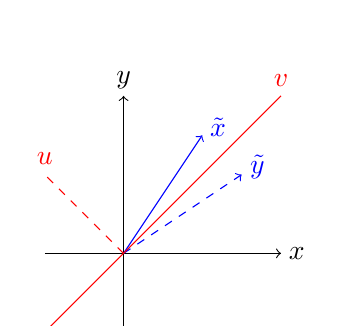
\begin{tikzpicture}
            \draw [-to] (0,-1) -- (0,2);
            \draw [-to] (-1,0) -- (2,0);
            \draw [-to,blue] (0,0) -- (1,1.5);
            \draw [-to,blue,dashed] (0,0) -- (1.5,1);
            \draw [red,dashed] (0,0) -- (-1,1);
            \draw [red] (-1,-1) -- (2,2);
            \node [blue] at (1.2,1.6) {$\tilde{x}$};
            \node [blue] at (1.7,1.1) {$\tilde{y}$};
            \node at (2.2,0) {$x$};
            \node at (0,2.2) {$y$};
            \node [red] at (-1,1.2) {$u$};
            \node [red] at (2,2.2) {$v$};
        \end{tikzpicture}
    \end{center} 
    

    \[H\tilde{x} = \tilde{y}~~~~~~\]

    \[Hu = -u~~~~~~\]

    \[Hv = v~~~~~~\]

\end{multicols}

\

Como $v$ y $u$ forman una base, entonces $\tilde{x} = \alpha v + \beta u$. Además, la reflexión de $\tilde{x}$ es $\tilde{y} = \alpha v - \beta u$.

Entonces, buscamos $H$ tal que $H\tilde{x} = \alpha v - \beta u$
\[\alpha v - \beta u = \alpha v + \beta u - 2\beta u\]
\[H\tilde{x} = I\tilde{x} - W\tilde{x} ~~\text{tal que}~~ W\tilde{x} = \alpha Wv + \beta Wu = 2\beta u\]

y se necesita que $Wv = 0$ y $Wu = 2u$.

\

\noindent Sea $P = uu^t$ y asumamos ${||u||}_{2} = 1$, tenemos que

\begin{itemize}
    \item[-] $P$ es simétrica.
    \item[-] $PP^t = P$.
    \item[-] $Pu = u$.
    \item[-] $Pv = 0$.
\end{itemize}

\noindent Si definimos $W = 2P$, se tiene

\[H = I - 2P\]
\[H\tilde{x} = (I-2P)(\alpha v + \beta u) =\]
\[I(\alpha v + \beta u) - 2P(\alpha v + \beta u) =\]
\[\alpha v + \beta u - 2\beta u = \tilde{y}\]



\subsubsection{Propiedades de H}\label{subsubsec:householder_propiedades_h}

\[H = I - 2uu^t\]

\begin{itemize}
    \item[-] $H$ es simétrica.
    \item[-] $H$ es ortogonal.
\end{itemize}

\

\noindent Sean $\tilde{x},~\tilde{y} \in \mathbb{R}^{n},~\tilde{x} \neq \tilde{y},~{||\tilde{x}||}_{2} = {||\tilde{y}||}_{2}$. Existe una transformación de Householder tal que $H\tilde{x} = \tilde{y}$.

\

\begin{multicols}{2}
    \begin{center}    
        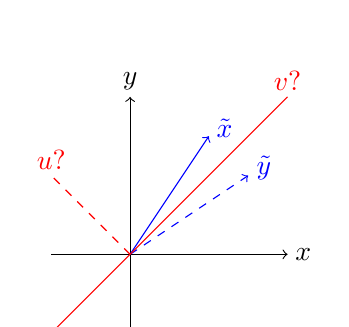
\begin{tikzpicture}
            \draw [-to] (0,-1) -- (0,2);
            \draw [-to] (-1,0) -- (2,0);
            \draw [-to,blue] (0,0) -- (1,1.5);
            \draw [-to,blue,dashed] (0,0) -- (1.5,1);
            \draw [red,dashed] (0,0) -- (-1,1);
            \draw [red] (-1,-1) -- (2,2);
            \node [blue] at (1.2,1.6) {$\tilde{x}$};
            \node [blue] at (1.7,1.1) {$\tilde{y}$};
            \node at (2.2,0) {$x$};
            \node at (0,2.2) {$y$};
            \node [red] at (-1,1.2) {$u?$};
            \node [red] at (2,2.2) {$v?$};
        \end{tikzpicture}
    \end{center} 

    \[v = \tilde{x} + \tilde{y}~~~~~~\]

    \[u = \frac{\tilde{x} - \tilde{y}}{{||\tilde{x}-\tilde{y}||}_{2}}~~~~~~\]

    \[H = I - 2\frac{(\tilde{x}-\tilde{y}){(\tilde{x}-\tilde{y})}^{t}}{{||\tilde{x}-\tilde{y}||}_{2}^{2}}~~~~~~\]
\end{multicols}



\noindent Sean $A \in \mathbb{R}^{2 \times 2},~\tilde{x}=\begin{bmatrix}
    a_{11} \\ a_{21}
\end{bmatrix}$ y $\tilde{y} = \begin{bmatrix}
    {||\tilde{x}||}_{2} \\ 0
\end{bmatrix}$.

\

\noindent Existe $H$ tal que $H\tilde{x} = \tilde{y}$.

 \[HA = \begin{bmatrix}
    {||\tilde{x}||}_{2} & * \\
    0 & *
 \end{bmatrix}\]
 \[HA = R\]
 \[H^{t}HA = H^{t}R\]
 \[A = QR\]

\subsubsection{Costo}\label{subsubsec:householder_costo}

\subsubsection{Ejemplo}\label{subsubsec:householder_ejemplo}

\subsection{Propiedades}\label{subsec:propiedades_qr}
\newpage

\end{document}
